%%%%%%%%%%%%%%%%%%%%%%%%%%%%%%%%%%%%%%%%%
% Wenneker Article
% LaTeX Template
% Version 2.0 (28/2/17)
%
% This template was downloaded from:
% http://www.LaTeXTemplates.com
%
% Authors:
% Vel (vel@LaTeXTemplates.com)
% Frits Wenneker
%
% License:
% CC BY-NC-SA 3.0 (http://creativecommons.org/licenses/by-nc-sa/3.0/)
%
%%%%%%%%%%%%%%%%%%%%%%%%%%%%%%%%%%%%%%%%%

%----------------------------------------------------------------------------------------
%	PACKAGES AND OTHER DOCUMENT CONFIGURATIONS
%----------------------------------------------------------------------------------------

\documentclass[11pt, a4paper]{article} % 10pt font size (11 and 12 also possible), A4 paper (letterpaper for US letter) and two column layout (remove for one column)

\usepackage[english]{babel} % English language hyphenation
\usepackage{microtype} % Better typography
\usepackage{amsmath,amsfonts,amsthm} % Math packages for equations
\usepackage[svgnames]{xcolor,colortbl} % Enabling colors by their 'svgnames'
\usepackage[hang, small, labelfont=bf, up, textfont=it]{caption} % Custom captions under/above tables and figures
\usepackage{booktabs} % Horizontal rules in tables
\usepackage{lastpage} % Used to determine the number of pages in the document (for "Page X of Total")
\usepackage{graphicx} % Required for adding images
\usepackage{amssymb}
\usepackage[mathscr]{eucal}
\usepackage[table]{xcolor}
\usepackage{enumitem} % Required for customising lists
\setlist{noitemsep} % Remove spacing between bullet/numbered list elements
\usepackage{sectsty} % Enables custom section titles
\allsectionsfont{\usefont{OT1}{phv}{b}{n}} % Change the font of all section commands (Helvetica)
\usepackage{hyperref}
\usepackage[sort,numbers]{natbib}
\usepackage{fancyhdr}
\usepackage{url}
\usepackage{floatrow}

\definecolor{Gray}{gray}{0.85}
\definecolor{LightCyan}{rgb}{0.88,1,1}
\definecolor{LightPink}{rgb}{0.25,0.5,1}
\definecolor{bubblegum}{rgb}{0.99, 0.76, 0.8}
\definecolor{pastelpink}{rgb}{1.0, 0.82, 0.86}
\definecolor{piggypink}{rgb}{0.99, 0.87, 0.85}
\definecolor{pink}{rgb}{1, 0.5, 0.9}
\definecolor{lightpink}{rgb}{1.0, 0.61, 0.76}

% ----------------------------------------------------------------------------------------
%	MARGINS AND SPACING
%----------------------------------------------------------------------------------------
\usepackage{geometry} % Required for adjusting page dimensions
\geometry{
	top=1.5cm, % Top margin
	bottom=1.5cm, % Bottom margin
	left=1.5cm, % Left margin
	right=1.5cm, % Right margin
	includehead, % Include space for a header
	includefoot, % Include space for a footer
	%showframe, % Uncomment to show how the type block is set on the page
}
\setlength{\columnsep}{6mm} % Column separation width

%----------------------------------------------------------------------------------------
%	FONTS
%----------------------------------------------------------------------------------------

\usepackage[T1]{fontenc} % Output font encoding for international characters
\usepackage[utf8]{inputenc} % Required for inputting international characters
\usepackage{XCharter} % Use the XCharter font
\usepackage{verbatim} 
%\usepackage{fontspec}
%\setmainfont{TeX Gyre Termes}
\pagestyle{headings}
\usepackage{fancyhdr}
\setlength{\headheight}{15.2pt}
\pagestyle{fancy}
%%%%%%%%%%%%%%%%%%%%%%%%%%%%%%%%%%%%%%%%%%
% Wenneker Article
% Structure Specification File
% Version 1.0 (28/2/17)
%
% This file originates from:
% http://www.LaTeXTemplates.com
%
% Authors:
% Frits Wenneker
% Vel (vel@LaTeXTemplates.com)
%
% License:
% CC BY-NC-SA 3.0 (http://creativecommons.org/licenses/by-nc-sa/3.0/)
%
%%%%%%%%%%%%%%%%%%%%%%%%%%%%%%%%%%%%%%%%%

%----------------------------------------------------------------------------------------
%	PACKAGES AND OTHER DOCUMENT CONFIGURATIONS
%----------------------------------------------------------------------------------------

\usepackage[english]{babel} % English language hyphenation

\usepackage{microtype} % Better typography

\usepackage{amsmath,amsfonts,amsthm} % Math packages for equations

\usepackage[svgnames]{xcolor} % Enabling colors by their 'svgnames'

\usepackage[hang, small, labelfont=bf, up, textfont=it]{caption} % Custom captions under/above tables and figures

\usepackage{booktabs} % Horizontal rules in tables

\usepackage{lastpage} % Used to determine the number of pages in the document (for "Page X of Total")

\usepackage{graphicx} % Required for adding images

\usepackage{enumitem} % Required for customising lists
\setlist{noitemsep} % Remove spacing between bullet/numbered list elements

\usepackage{sectsty} % Enables custom section titles
\allsectionsfont{\usefont{OT1}{phv}{b}{n}} % Change the font of all section commands (Helvetica)

%----------------------------------------------------------------------------------------
%	MARGINS AND SPACING
%----------------------------------------------------------------------------------------

\usepackage{geometry} % Required for adjusting page dimensions

\geometry{
	top=1cm, % Top margin
	bottom=1.5cm, % Bottom margin
	left=2cm, % Left margin
	right=2cm, % Right margin
	includehead, % Include space for a header
	includefoot, % Include space for a footer
	%showframe, % Uncomment to show how the type block is set on the page
}

\setlength{\columnsep}{7mm} % Column separation width

%----------------------------------------------------------------------------------------
%	FONTS
%----------------------------------------------------------------------------------------

\usepackage[T1]{fontenc} % Output font encoding for international characters
\usepackage[utf8]{inputenc} % Required for inputting international characters

\usepackage{XCharter} % Use the XCharter font

%----------------------------------------------------------------------------------------
%	HEADERS AND FOOTERS
%----------------------------------------------------------------------------------------

\usepackage{fancyhdr} % Needed to define custom headers/footers
\pagestyle{fancy} % Enables the custom headers/footers

\renewcommand{\headrulewidth}{0.0pt} % No header rule
\renewcommand{\footrulewidth}{0.4pt} % Thin footer rule

\renewcommand{\sectionmark}[1]{\markboth{#1}{}} % Removes the section number from the header when \leftmark is used

%\nouppercase\leftmark % Add this to one of the lines below if you want a section title in the header/footer

% Headers
\lhead{} % Left header
\chead{\textit{\thetitle}} % Center header - currently printing the article title
\rhead{} % Right header

% Footers
\lfoot{} % Left footer
\cfoot{} % Center footer
\rfoot{\footnotesize Page \thepage\ of \pageref{LastPage}} % Right footer, "Page 1 of 2"

\fancypagestyle{firstpage}{ % Page style for the first page with the title
	\fancyhf{}
	\renewcommand{\footrulewidth}{0pt} % Suppress footer rule
}

%----------------------------------------------------------------------------------------
%	TITLE SECTION
%----------------------------------------------------------------------------------------

\newcommand{\authorstyle}[1]{{\large\usefont{OT1}{phv}{b}{n}\color{DarkRed}#1}} % Authors style (Helvetica)

\newcommand{\institution}[1]{{\footnotesize\usefont{OT1}{phv}{m}{sl}\color{Black}#1}} % Institutions style (Helvetica)

\usepackage{titling} % Allows custom title configuration

\newcommand{\HorRule}{\color{DarkGoldenrod}\rule{\linewidth}{1pt}} % Defines the gold horizontal rule around the title

\pretitle{
	\vspace{-30pt} % Move the entire title section up
	\HorRule\vspace{10pt} % Horizontal rule before the title
	\fontsize{32}{36}\usefont{OT1}{phv}{b}{n}\selectfont % Helvetica
	\color{DarkRed} % Text colour for the title and author(s)
}

\posttitle{\par\vskip 15pt} % Whitespace under the title

\preauthor{} % Anything that will appear before \author is printed

\postauthor{ % Anything that will appear after \author is printed
	\vspace{10pt} % Space before the rule
	\par\HorRule % Horizontal rule after the title
	\vspace{20pt} % Space after the title section
}

%----------------------------------------------------------------------------------------
%	ABSTRACT
%----------------------------------------------------------------------------------------

\usepackage{lettrine} % Package to accentuate the first letter of the text (lettrine)
\usepackage{fix-cm}	% Fixes the height of the lettrine

\newcommand{\initial}[1]{ % Defines the command and style for the lettrine
	\lettrine[lines=3,findent=4pt,nindent=0pt]{% Lettrine takes up 3 lines, the text to the right of it is indented 4pt and further indenting of lines 2+ is stopped
		\color{DarkGoldenrod}% Lettrine colour
		{#1}% The letter
	}{}%
}

\usepackage{xstring} % Required for string manipulation

\newcommand{\lettrineabstract}[1]{
	\StrLeft{#1}{1}[\firstletter] % Capture the first letter of the abstract for the lettrine
	\initial{\firstletter}\textbf{\StrGobbleLeft{#1}{1}} % Print the abstract with the first letter as a lettrine and the rest in bold
}

%----------------------------------------------------------------------------------------
%	BIBLIOGRAPHY
%----------------------------------------------------------------------------------------

\usepackage[backend=bibtex,style=authoryear,natbib=true]{biblatex} % Use the bibtex backend with the authoryear citation style (which resembles APA)

\addbibresource{example.bib} % The filename of the bibliography

\usepackage[autostyle=true]{csquotes} % Required to generate language-dependent quotes in the bibliography
 % Specifies the document structure and loads requires packages
\fancyhf{}
%\fancyhead[LE,RO]{Overleaf}
%\fancyhead[RE,LO]{Guides and tutorials}
%\fancyfoot[LO,RE]{FETOPEN-01 template WP18-20 v20171106}
\fancyfoot[LE,RO]{$\mathcal{ROBHOOT}$}
%\fancyfoot[LE,RE]{\thepage} % pa
\fancyfoot[L]{\thepage}
%----------------------------------------------------------------------------------------
%	ARTICLE INFORMATION
%----------------------------------------------------------------------------------------
\begin{document}

%\title{$\mathcal{ROBHOOT}$ \\ Open Discovery Network \\ v.1.0}} % The article title
\title{$\mathcal{ROBHOOT}$ \\ Discovery Knowledge Graphs in Evolutionary Biology-Inspired Federated Networks \\ v.2.0}}
%Automated discovery-knowledge graphs in federated heterogeneous networks
%Evolving Information processing systems in heterogeneous federated networks

%Automated Discovery Knowledge Graphs in Evolving Heterogeneous Federated Networks

%Biology-inspired information processing in large-scale heterogeneous federated networks

%The article title
  %\author{{\textsuperscript{1,2,3} and XY\textsuperscript{2,3}}% Authors
  \newline\newline % Space before institutions
  \\
%	\textsuperscript{1}\institution{}\\ % Institution 1
%	\textsuperscript{2}\institution{}\\ % Institution 2
	%\textsuperscript{3}\institution{\texttt{LaTeXTemplates.com}}
      %} % Institution 3


% Example of a one line author/institution relationship
%\author{\newauthor{John Marston} \newinstitution{Universidad Nacional Autónoma de México, Mexico City, Mexico}}

\date{\today} % Add a date here if you would like one to appear underneath the title block, use \today for the current date, leave empty for no date
%---------------------------------------------------------------------------------------

%\pagestyle{plain}
\maketitle % Print the title
%\thispagestyle{firstpage} % Apply the page style for the first page (no headers and footers)

\tableofcontents

%----------------------------------------------------------------------------------------
%	ABSTRACT
%----------------------------------------------------------------------------------------
\section*{{\bf Summary}} Global sustainability is a major goal of
humanity. Many studies have shown global sustainability could be
achieved by strengthening transparency, feedbacks and rapid access to
reproducible information among social, ecological, economical,
technological and governance systems. Sustainability goals, however,
strongly depend on global access to evidence-, and discovery-based
knowledge gaps. Yet, science-enabled technologies targeting global
knowledge gaps to reach sustainability and biodiversity conservation
goals are at a very incipient stage of development. We fussion data to
causal knowledge graph, the discovery knowledge graph, in evolutionary
biology-inspired federated networks for a sustainable- and
knowledge-inspired society. Discovery knowledge graphs running on a
federated network encompass a hybrid-technology to lay out the
foundation of an open- and cooperative-science ecosystem to automate
discovery in global emergency and sustainability challenges. The
project summarized here is not set out to deliver automated
discovery-knowledge graphs in evolving federated networks, but to
provide the architecture of a science-enabled technology, as a
proof-of-principle, to connect global human sustainability challenges
to knowledge-inspired societies.
%----------------------------------------------------------------------------------------
%	ARTICLE CONTENTS
% ----------------------------------------------------------------------------------------
\section{Excellence}
\subsection{Radical vision of a science-enabled technology}
We are in the midst of the fourth industrial revolution, a
transformation revolving around data driven intelligent machines and
knowledge-inspired societies. More than half of the global population
is now online using the Internet (i.e., 3.9 billion), which represents
a more inclusive global information society ({\bf +++}). The Internet
is rapidly evolving and people is using technology in powerful ways,
from adopting decentralized technologies for humanitarian efforts to
improving agricultural practices and reducing waste in the global food
supply chain (\citep{Wilson2018},+++). Data analytics is advancing at
the pace dictated by the availability of data and a myriad of
data-driven approaches are being developed to extract patterns from
data (\citep{Schmidhuber:2015}). Data analytics and the methods
developed around it is also being challenged because the diversity of
data is growing worldwide ({\bf +++}). On the other side, AI
approaches are rapidly evolving towards more explainable/interpretable
pattern description ({\bf +++}). This forces the digital ecosystem to
account for the increasing data heterogeneity and the need of novel
methods for finding rapidly interpretable patterns, but still,
science-enabled technologies accounting for data heterogeneity and
interpretable patterns are scarce \citep{RePEc}.\textcolor{red}{Still
  much bla bla -- more flow towards the main point}
  
\textcolor{red}{Describe how our vision surpasses substantially any
  technological paradigms that currently exist or are under
  development} The transformation of a digital society into a
knowledge-inspired society requires solving several gaps: First,
science-enabled technological paradigm assisting humans is biased
towards a limited range of the ``observable'' heterogeneity in
data-sources limiting the number of interpretable patterns ({\bf
  +++}). Second, the AI technological paradigm is rooted in
optimization functions (i.e., function loss or reward, similar to
fitness optima functions in evolutionary biology {\bf
  +++}). Optimization-based technologies limit a broader number of
plausible solutions, as usually found in evolving learning capable
biological systems ({\bf +++}), and third, science-enabled
technologies (for scientific inquiry) are highly fragmented, partly
solve reproducibility and are mostly developed in close-source
software
(\citep{Inhaber1977,Ioannidis2005,Fang2011,Gunther2018,Hardwicke2018,Mehrabi2019,Real2020}). To
leverage the abundance and heterogeneity of data, a science-enabled
technology should be able to obtain information from a large pool of
heterogeneous data-sources. Second, the analysis of the data should go
beyond the identification of patterns and consider approaches
delivering processes, the interpretable patterns, to the
end-user. Third, the analysis should be performed in federate way,
such that highly heterogeneous populations can learn from each other
to reach consensus about the population of plausible scenarios
accounting for data heterogeneity, and finally, the whole process
should be automated, reproducible and transparent such that benefit
the public.

\textcolor{red}{Describe the vision of a radically-new
  science-enabled technology that the project would contribute
  towards}The project will
% contribute towards automated discovery-knowledge graphs accounting
% for heterogeneous data-individuals-groups-societies interchanging
% functional information to reach partial solutions in the face of
% rapidly emerging global sustainability challenges.
In this regard, obtaining interpretable information from data
collected from many distinct sources combined with science-enabled
technologies accounting for evolving interactions among distinct
heterogeneous groups are required to gain more robust scenarios in
knowledge-inspired societies. Yet, discovery science-enabled
technologies delivering interpretable patterns from heterogeneous
data-sources applied to gain information of complex governance,
social, environmental and technological problems are particularly
lacking (Figure 1 and Table 1) \citep{Mastrangelo2019}. Our project
contributes towards a science-enabled technology accounting for data
heterogeneity and interpretable patterns, the discovery knowledge
graph (Figures 1 and 2 and Table 1), obtained from evolutionary
biology-inspired in federated networks. Evolutionary dynamics-inspired
technology extracting information from highly heterogeneous and
multidimensional groups while minimizing the need of having optimal
solutions makes possible the study of within and between groups
consensus scenarios to enrich knowledge-inspired societies facing
global challenging problems.

% Evolutionary computation models accounting for multidimensionality
% and node heterogeneity are rare
Many experimental evolution and evolutionary computation models have
shown the plausibility of coexistence of multiple heterogeneous
populations ({\bf +++}). Many interpretable mechanisms have been
proposed to explain such a coexistence, like negative-frequency
dependent selection (Doebeli book and others, {\bf +++}),
fluctuating-selection, and many others ({\bf +++}). Yet, approaches
accounting for not optimal or maladaptive solutions in the context of
group heterogeneity in multidimensional landscapes are rare (refs
around evolution cooperation in multidimensional landscapes, {\bf
  +++}). In ecological systems, intraspecific trait variation (i.e., a
proxy for heterogeneity within a species) and trait dimensionality
(i.e., biotic, reproductive, abiotic and migration traits for example)
might be driving functional interactions with other species (i.e.,
cooperative, antagonistic, competitive, or mutualistic, infectious
diseases... etc), but most approaches have neglected the effect of
trait dimensionality in heterogeneous populations on interactions
being these competition or cooperation {\bf (On neural systems, the
  vast majority of neurons in the brain show highly differentitated
  morphological, genetic and phenotypic states? (refs, Wolfgang))},
yet the understanding of functional interactions among such a highly
differentiatied states (groups, etc) is not well understood. Taken
together, these results suggest that evolved information processing
systems formed by highly heterogeneous groups (refs about federated
networks, bacterial consortia, federated bacteria..., artificial life,
problem solving artificial societies, and large-scale meta-learning in
the federated setting \citep{Dilley2016}), is currently quite limited
and that new science-enabled technologies accounting for
diversification, dimensionality and heterogeneity of highly distinct
groups in functional information processing federated networks, are
required to develop further the increasing demand of data-source
heterogeneity and interpretable-knowledge patterns.

Biodiversity data collected by many different countries is a good
example for understanding open-problems in federated networks. Many
international programs for exploration of the seas (i.e., ICES, ...)
involve many countries collecting biodiversity data using, despite
efforts of standarization, different protocols and technologies. The
data is then used to understand the spatiotemporal dynamics of the
ecological communities as a baseline to inform fisheries ({\bf
  +++}). Each country might collect data with different gear systems
(Figure 2). This is because each country has commercial interests in
specific species, despite attempts to dictate standards for the gear
systems among all the countries. The result is that countries use
different gear systems and collect heterogeneous and biased data about
the same species. This makes difficult to obtain accurate distribution
maps of species (Figure 2). This situation can be outlined as follows:
country own's interest in specific gear systems vs. shared interest
using standarized gears to share more accurate species and communities
maps (i.e., a problem similar to the tragedy of commons, {\bf
  +++}). This last one strategy is built on cooperation between two
countries to understand better a specific species while sacrificing
their own commercial interest (Figure 2). This is a common situation
when many heterogeneous nodes (i.e., countries with different
interests, groups, funding and conservation strategies, etc) exploit
resources (i.e., species within ecosystems compossed by a network of
interacting species compossed by heterogeneous individuals within and
between species, food webs, mutualistic networks, etc) using different
technologies (i.e., gear systems). Many of these ecosystems are
overexploited and yet science-based technologies providing forecasting
scenarios accounting for heterogeneous biodiversity data (i.e.,
species and environment), sampling protocols (i.e., many gear systems
and other technologies), and groups (i.e., within and between
countries) to mitigate risks and enhance global cooperation scenarios
in such a multidimensional ecosystems are not in place
(\citep{Wilson2018}, {\bf +++}).

\textcolor{red}{Describe the overall and specific objectives for the
  project, which should be clear, measurable, realistic and achievable
  within the duration of the project. (The details of the project plan
  belong to the Implementation section)} The example about the
exploration of the seas teaches us the need of science-enabled
technologies facilitating interpretable patterns accounting for
heterogeneous data and groups to overcome fragmented and partial
responses to a global biodiversity problem. The goal of
$\mathcal{ROBHOOT}$ is to propose a science-enabled technology concept
integrating data and causal knowledge graphs into evolutionary
biology-inspired federated networks to lay the foundation for a novel
scientific discovery technology. $\mathcal{ROBHOOT}$ contributes
towards reproducible cooperative forecasting scenarios in rapidly
changing global sustainability landscapes (Figures 1, 2, and 3): {\bf
  $\mathcal{ROBHOOT}$ v.1.0} deploys data knowledge graphs obtained
from heterogeneous data-sources to decipher global data-architecture
maps. {\bf $\mathcal{ROBHOOT}$ v.2.0} develops explainable
evolutionary biology-inspired approaches to fussion data and causal
knowledge graphs into discovery knowledge graphs, and {\bf
  $\mathcal{ROBHOOT}$ v.3.0} expands discovery knowledge graphs along
evolutionary biology-inspired federated networks.

\begin{figure}[h!]
    \hspace{-0.25 in}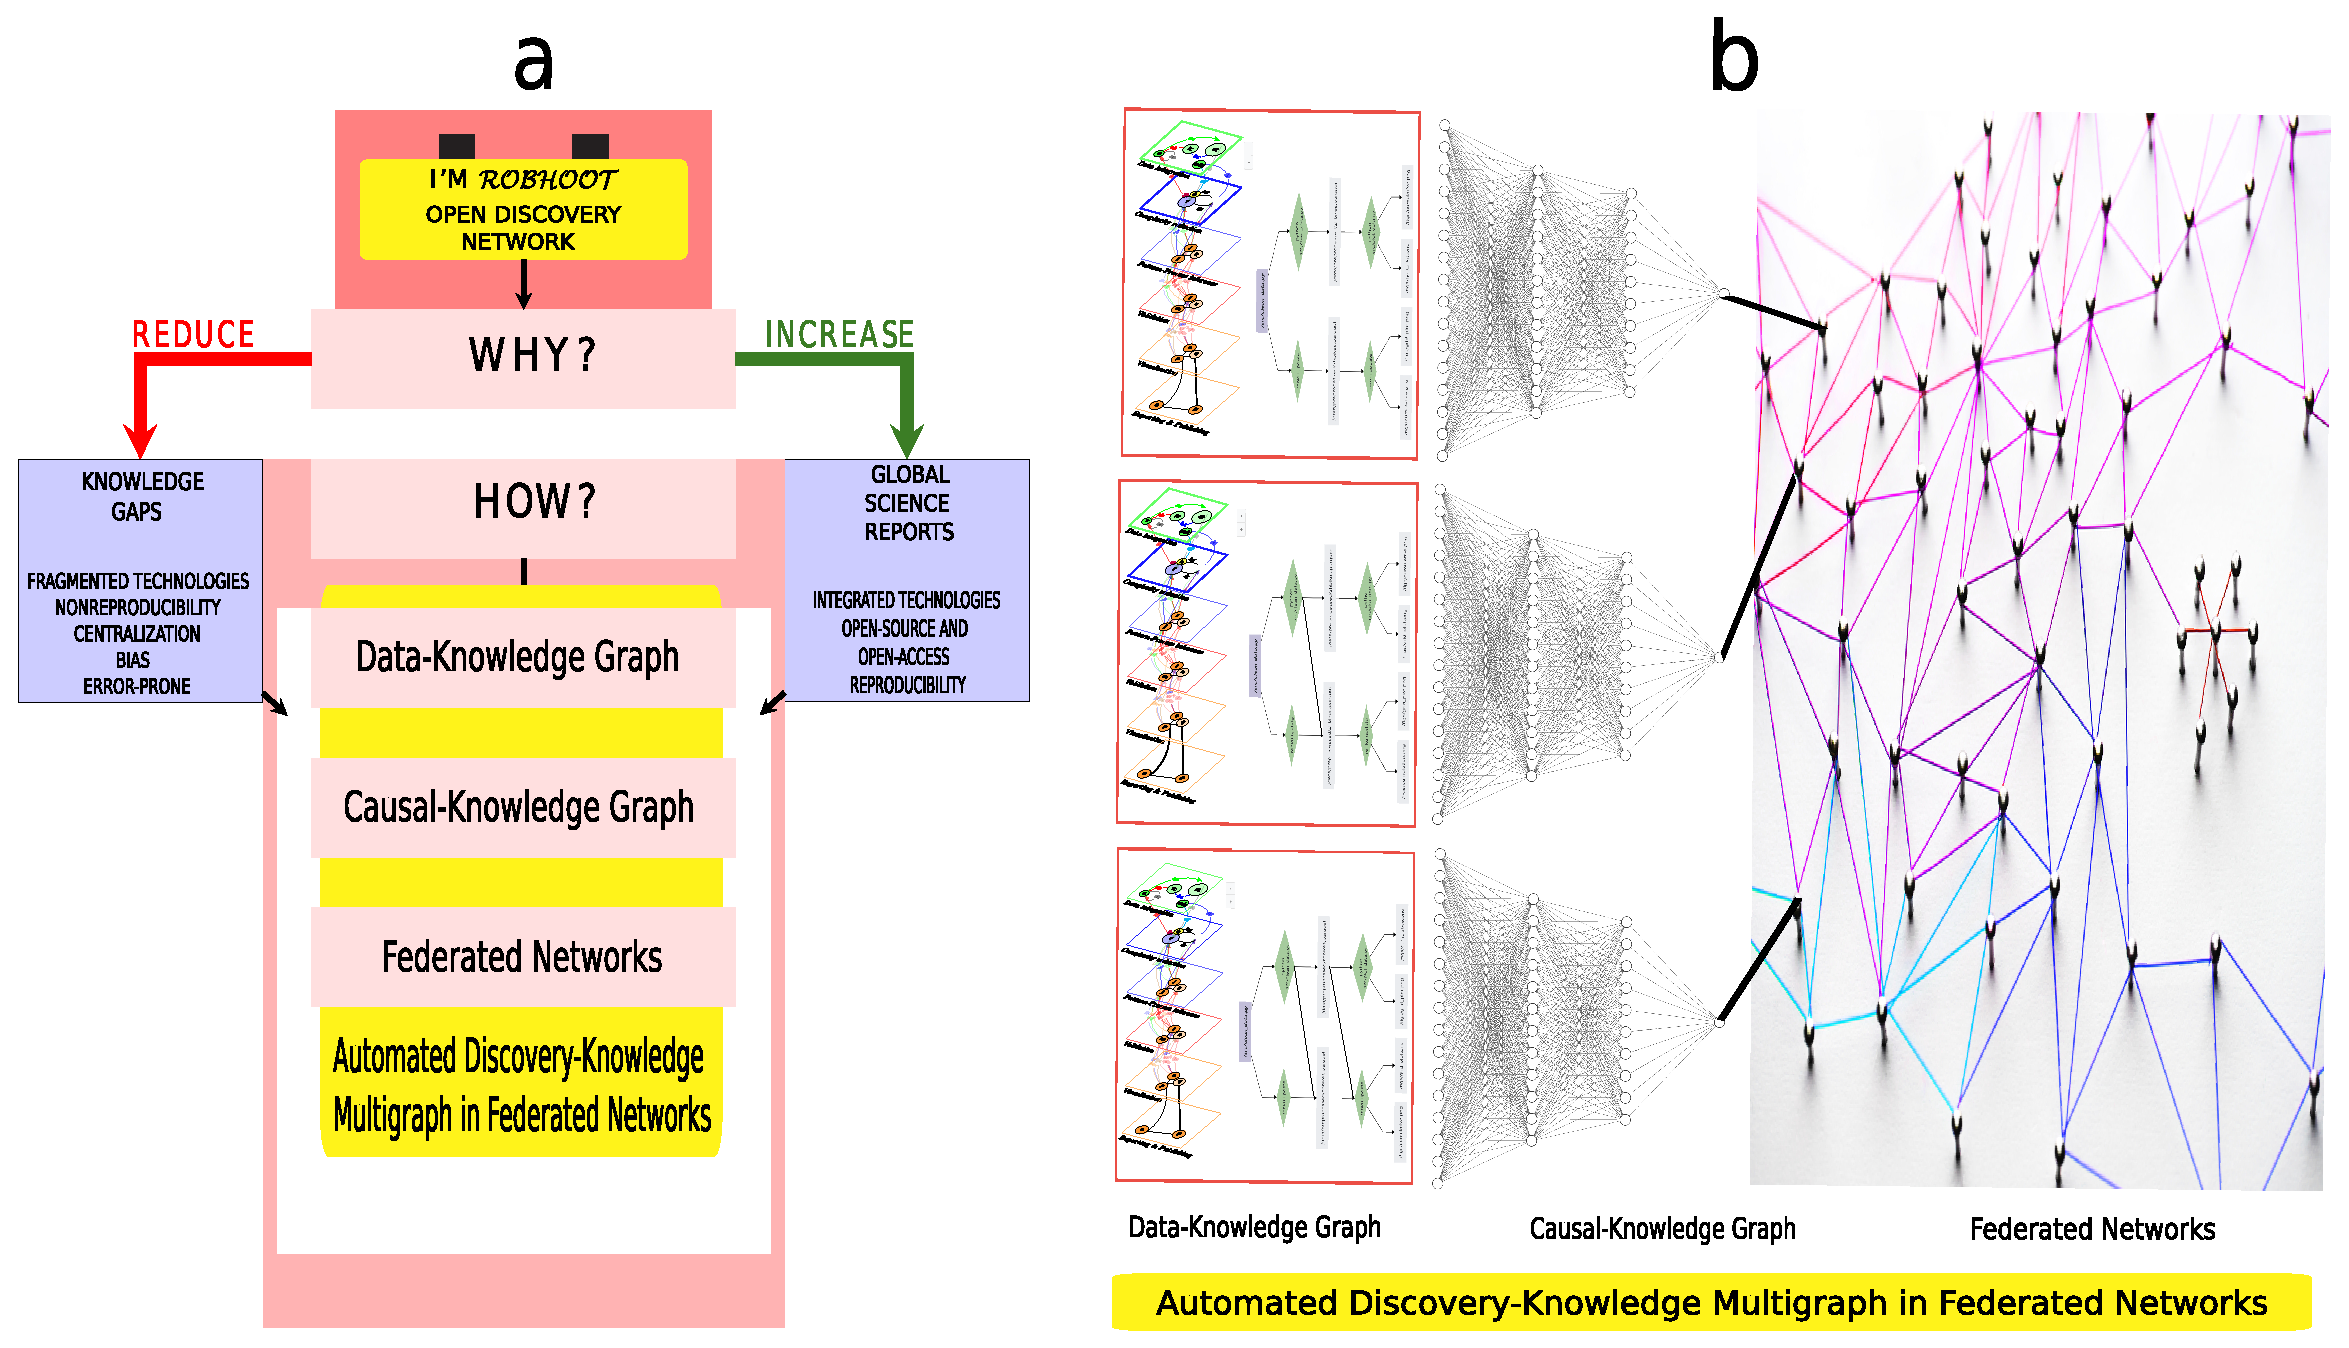
\includegraphics[width=1\textwidth]{Figures/AutomatedDiscovery.pdf}
    \caption*{\small {\bf Figure 1: Discovery in Evolutionary
        Biology-Inspired Federated Networks}. $\mathcal{ROBHOOT}$
      fussion data and causal knowledge graphs, the ``Discovery
      Knowledge Graphs'', into biology-inspired federated networks for
      a sustainable knowledge-inspired society: {\bf a)}
      $\mathcal{ROBHOOT}$ targets global knowledge gaps (red path) and
      open-access reproducible discovery reports (green path). It
      integrates three science-enabled technologies: {\bf a,b)} Data
      Knowledge Graphs for heterogeneous source-data discovery. {\bf
        a,b)} Causal Knowledge Graphs to fussion data knowledge to
      interpretable patterns using ``Evolutionary AI automation'' and
      biology-inspired methods, and {\bf a,b)} Discovery in
      biology-inspired federated networks for ``Cooperative
      Forecasting''. {\bf Discovery knowledge graphs in
        biology-inspired federated networks} integrate data and causal
      knowledge graphs into federated networks to generate cooperative
      forecasting to respond to global and sustainability
      challenges.}}
\end{figure}

%--------------------Currently out of the draft
\begin{comment}
 The Robhoot project is trying to introduce new concepts to allow
  scientist and the public to interact in a decentralized open-access
  knowledge network to gain informed decisions when solving complex
  social, environmental and technological problems. Current
  technologies for scientific inquiry are highly fragmented and thus
  only increase robustness, reproducibility and the interactions with
  the public marginally (refs). The goal of Robhoot is to propose a
  new hybrid-technology concept combining deep learning, automation
  and distributed ledger technology with the advances of neural
  biological networks to lay the foundation for a novel open-science
  ecosystem aiming to couple predictive and knowledge power in
  contemporary societies. Robhoot is not set out to deliver a finished
  deep knowledge ledger network in the science ecosystem but provide a
  science-enabled technology in establishing a prototype
  proof-of-principle for an open public-science ecosystem.
 
\begin{table}
 %\rowcolor{pink}
\begin{tabular}{ p{6cm} | p{3cm} | p{3cm}}
  \hline \hline
  \textbf{Features} & \textbf{Science Ecosystem} &\textbf{{\bf $\mathcal{ROBHOOT}$}}\\  \hline
  Decentralization & No & Yes \\ \hline
  Full automation & No & Yes \\ \hline
  Open-access & Mostly No & Yes \\ \hline
  Immutability & No & Yes \\ \hline
  Robustness & Mostly No & Yes \\ \hline
  Reproducibility & Mostly No & Yes \\ \hline        
  Owner-Controlled assets & No & Yes \\ \hline       
  \bottomrule
\end{tabular}
\caption{{\bf $\mathcal{ROBHOOT}$} is designed to resolve desirable
  properties of science: Open-access, immutability, robustness,
  reproducibility, and owner-controlled assets. These features will be
  added during the different stages of development of the project
  (section ``Design Goals'').}
\end{table}
\end{comment}
%-----------------------------------------------------------------

   
\begin{table*}[ht]
 %\rowcolor{pink}
\begin{tabular}{ p{6cm} | p{11cm}}
  \hline \hline
  \textbf{Word} &\textbf{Meaning}\\  \hline
  Data knowledge graph & Technology-driven information extraction from heterogeneous data-sources  \\ \hline
  Causal knowledge graph & Technology-driven explainable/interpretable patterns to take better informed decisions on global and complex sustainability challenges\\ \hline
  % Evidence-based knowledge gap & Solid scientific knowledge facing
  % constraints to be transfered to benefit society\\ \hline
  % Research-based knowledge gap & Differential access to the research
  % knowledge limiting information transfer to the society \\ \hline
  Discovery knowledge graph & Fussion of data and causal knowledge graphs for better pattern understanding of heterogeneous data\\ \hline
  %Reproducible knowledge graph & High-resolution tracking of the research cycle to make it fully open and transparent\\ \hline
  Automation & Algorithms targeting minimal human-driven interference\\ \hline
  Knowledge inspired society & Open-access discovery to facilitate informed decisions in global sustainability challenges \\ \hline
  Neutral-knowledge generation & Reproducible reports making transparent the many sources of bias in the discovery process\\ \hline
  \bottomrule
\end{tabular}
\caption{{\bf Glossary of terms.}}
\end{table*}

\subsection{Science-to-technology breakthrough that addresses this vision}

Interconnected global societies are constantly facing new challenges
that need to be rapidly addressed. In this regard, technologies
integrating data-driven causal inference into intelligent networks
providing rapid and global interpretable information when solving
complex governance, social, environmental and technological problems
are lacking. Depite rapid advances of research platforms for data
analytics in the last decade
\citep{Melniketal:2010,Steinruecken,Modulos,Guimera2020,GoogleAI,IrisAI,easeml,datarobot,aito},
the integration of science-enabled technologies currently lack
knowledge-inspired approaches accounting for data heterogeneoity and
interpretable pattern discovery impacting knowledge-inspired societies
to help responding to rapidly evolving global sustainability
challenges (Figures 1 and 2, and Table 1). Technologies facilitating
interpretable patterns from complex systems accounting for large
heterogeneity and multidimensionality present still many challenges
({\bf +++}). This is particularly relevant in global emergency or
sustainability landscapes, where data heterogeneity properties like
availability, data fragmentation, and transparency drive constantly
emerging feedbacks among the many data-sources to predict new
situations more accurately (Figure 2).

Our understanding of evolved information processing systems driven by
multidimensional factors and highly heterogeneous groups is currently
quite limited. \textcolor{red}{Discuss the relevant state-of-the-art
  and the extent of the advance the project would provide beyond this
  state-of-the-art. How will $\mathcal{ROBHOOT}$ go beyond
  state-of-the-art? $\mathcal{ROBHOOT}$ introduces biology-inspired
  explainable knowledge graphs into federated networks accounting for
  heterogeneity and multidimensionality to make discovery a rapidly
  evolving feature in digital ecosytems (Figure 2). How will
  $\mathcal{ROBHOOT}$ explicitly deal with diversification and
  dimensionality when accounting for highly heterogeneous evolving
  groups and interactions? (refs about federated networks, bacterial
  consortia, federated bacteria..., artificial life, problem solving
  artificial societies, and large-scale meta-learning in the federated
  setting \citep{Dilley2016}). Describe the science-to-technology
  breakthrough, targeted by the project that would represent the first
  proof of concept of the envisioned technology.} Patterns from
knowledge-graphs are emerging at a fast pace in specific frontiers
{\bf +++}, but remains isolated from the discovery process especially
in the context of cooperative discovery in federated networks {\bf
  +++}. $\mathcal{ROBHOOT}$ goes beyond the state-of-the-art of
knowledge-graphs by fussioning data and causal knowledge graphs, the
discovery knowledge graphs, and scalating these into evolving
biology-inspired federated networks to move knowledge-inspired
societies towards reaching global sustainability goals when large
number heterogeneous groups share resources driven by multiple
factors.}

{\bf $\mathcal{ROBHOOT}$ v.1.0} deploys a data discovery technology to
generate data knowledge graphs for an understanding of interpretable
patterns accounting for heterogeneous data-sources. Data-architecture
alone is not sufficent to outline predictive scenarios in complex
sustainability problems. Therefore, data analytics complementing
data-architecture discovery is desirable to interpret scenarios in
natural and digital ecosystems. In this regard, there are also many
gaps in connecting global data-architecture into rapid automated
causal knowledge graphs, the discovery knowledge graphs, to facilitate
discovery. {\bf $\mathcal{ROBHOOT}$ v.2.0} integrates automated and
explainable evolutionary biology-inspired methods to decipher causal
knowledge graphs from open-ended modeling scenarios. Still, rapidly
drawing scenarios from a few labs limit the parameter phase space from
where the discovery process is generated. Therefore, the scalability
of fully reproducible discovery strongly depend on cooperation and
learning in large scale biology-inspired federated networks. {\bf
  $\mathcal{ROBHOOT}$ v.3.0} brings discovery knowledge graphs to
federated networks by connecting heterogeneous-neural inspired
networks to learning to obtain cooperative forecasting from
heterogeneous collections of data-sources (section 3.3).

\subsection{Interdisciplinarity and non-incrementality of the research
  proposed}

\textcolor{red}{Respond more directly! --- Explain why the proposed
  research is non-incremental --- Describe the research disciplines
  necessary for achieving the targeted breakthrough of the project and
  the added value from the interdisciplinarity:: Still in a
  descriptive phase here:: Now it is a disconnected set of ideas} {\bf
  $\mathcal{ROBHOOT}$} is a science-enabled multi-feature technology
for interpretable data-driven discovery in federated networks (Figures
1 to 3 and Tables 1 to 3). It contains three milestones each
characterized by a mixture of research disciplines. {\bf
  $\mathcal{ROBHOOT}$ v.1.0} is composed by computer scientists,
evolutionary biologists and developers targeting novel evolutionary
inspired algorithms for API data discovery. This module is
complemented with scientists from complex networks taking care of
quantitative methods in the data knowledge graphs to decipher the
existing gaps in data discovery and data-architecture technologies
(section 3.1). {\bf $\mathcal{ROBHOOT}$ v.2.0} team is compossed by
data-scientists trained in deep learning networks and automation
algorithms, theoreticians and biologists with expertise in modeling
mechanistic and Bayesian networks and biology-inspired neural
networks, respectively. The combination of data-scientists,
theoreticians and biologists generates a diverse team targeting
synthesis between automated and explainable evolutionary
biology-inspired approaches to decipher causal knowledge graphs from
heterogeneous data-sources (section 3.2). {\bf $\mathcal{ROBHOOT}$
  v.3.0} combines computer scientists and developers targeting sharing
and evolutionary biology-inspired models of federated networks, with
social scientist, and scientists specialized in ecology and
evolutionary biology (section 3.3). The complementarity of the teams
in modules one to three strengthen the collaboration for making
$\mathcal{ROBHOOT}$ a science-enable functional technology in a
rapidly evolving digital ecosystem \citep{Soto-Valero2019}.

\textcolor{red}{$\mathcal{ROBHOOT}$ aims to bring global transparency
  in knowledge generation by acting as an assistant or as an automated
  and reproducible discovery generator to facilitate sustainability
  goals in ecosystems. The multi-feature, science-enabled technology
  target a reduction in global knowledge gaps while transparently
  accounting for centralization \citep{Inhaber1977,Gunther2018}⁠⁠, bias⁠⁠
  \citep{Ioannidis2005}, error-prone \citep{Fang2011}, and
  non-reproducibility \citep{Hardwicke2018} (Figures 1 and 2 and Table
  1). These features are mostly due to the rapidly evolving digital
  ecosystem. For example, it is increasing continuously its computing
  capacity, new methods integrating automated and explainable AI are
  rapidly advancing, and their interconnection to open-source
  technologies is also rapidly occurring in the digital ecosystem {\bf
    +++}. Yet, targeting automated data and causal knowledge graphs
  into federated networks still require taking risky steps: combining
  heterogeneous data-sources and evolutionary biology-inspired neural
  modeling approaches to fill out the existing gaps in the explainable
  methods arena ato bring them to causal inference of learning with
  heterogeneous agents sharing resources in complex ecosystems.}

  \begin{comment}
  Yet, technologies with the capacity to compactly accounting for neutral,
  borderless, immutable, and open-access information in hybrid,
  trusted-untrusted peer-to-peer interactions, accounting for the
  multilayer nature of science and engineering are currently not in
  place. We have already advanced in the integration of the different
  modules, from the automated identification, retrieval and data
  integration to inference and process-based discovery. We have
  implemented a prototype for the ongoing covid-19 pandemic (section
  3.3). Each module includes state-of-the-art developments in computer
  science, complex systems, and theoretical evolutionary ecology. The
  proof- of-concept is not fully automated yet and still requires
  human intervention in module integration and the development of a
  testnet stage. Nonetheless, we are currently exploring innovative
  solutions especially in the modules of automated data discovery,
  causal-knowledge graphs, reporting, and visualization.  Producing
  such a technology will require integrating expertise from disparate
  disciplines like multilayer networks, deep learning, automation
  algorithmics, and distributed technologies. The integration of these
  disciplines will require to go beyond domain boundaries.
\end{comment}

%Renku, Fabric and gitchain.

\subsection{High risk, plausibility and flexibility of the research approach}


\begin{itemize}
\item \textcolor{red}{Explain how the research approach relates to the
    project objectives and how it is suitable to deal with the
    considerable science-and-technology uncertainties and appropriate
    for choosing alternative directions and options. (The risks and
    mitigation plan should be spelled out under the Implementation
    section).}
\end{itemize}

\begin{comment}
  Knowledge-inspired societies and governance will demand full
  research cycle transparency, reproducibility and interpretability to
  inform complex social, environmental and technological problems. The
  need of transparency, reproducibility and interpretability brings
  many technical and functional challenges to our research proposal
  because obtaining robust knowledge from integrating many parts each
  containing its own set of methods can generate divergent, fragile
  and contradictory outcomes. {\bf $\mathcal{ROBHOOT}$} will have a
  modular and flexible structure following four main versions each
  divided in four work packages and milestones.
\end{comment}

\begin{comment}
  We will develop a flexible research method focusing more in the
  algorithmic robustness of the deep ledger knowledge network than in
  the development of robust automated knowledge generation. Our
  motivation will be to provide a first proof of concept of how the
  technology works: we will sample the KGs using different deep
  learning algorithms to estimate the uncertainty of the ruled-based
  inference obtained by fitting predictions to simulated data (Goal
  G1). Accounting for the uncertainties of each of the research stages
  when sampling the KGs comes from the many distinct paths within and
  across the layers in the research cycle (Figure 1). We will test a
  variety of consensus algorithms to explore the degree of security,
  decentralization and scalability of the ledger knowledge network
  using the generated population of KGs (Goal G2). Despite our focus
  will be bias towards the side of the algorithmic robustness of the
  deep ledger knowledge network, we will develop a domain-specific
  case study, our Robhoot Open Network, to test the robustness of the
  rule-based inference obtained by fitting each of the generated KG to
  the empirical patterns (Goal G3). The high risk associated to
  robustly automate the full research cycle for producing immutable
  open knowledge is buffered to a great extend because the existing
  ecosystem of tested and reliable open-source tools: We will combine
  our own algorithms (i.e., data integration and deep learning
  algorithms for sampling and automating the KGs) with open-source
  tools like Renku, Fabric and gitchain. This open-ecosystem will
  allow us to have a flexible launching of a testnet to collect data
  to explore the security-scalability-decentralization patterns and
  the robustness of the generated KGs in the deep ledger knowledge
  network (Goal G4.)
\end{comment}



%============IMPACT====================================================
\section{Impact}
\label{cha:impact}


\subsection{Expected impact} 
\label{sec:expected-impact}
\instructions{
  \textit{Please be specific, and provide only information that applies to the proposal and its objectives. Wherever possible, use quantified indicators and targets.}\\

  \textcolor{red}{Describe how the project will contribute to the
    expected impacts set out in the work programme under the relevant
    topic: Scientific and technological contributions to the
    foundation of a new future technology:: Describe the importance of
    the technological outcome with regards to its transformational
    impact on science, technology and/or society:: Building leading
    research and innovation capacity across Europe by involvement of
    key actors that can make a difference in the future, for example
    excellent young researchers, ambitious high-tech SMEs or
    first-time participants to FET under Horizon 2020:: FET Open
    combines high scientific ambition with concrete technological
    implications. It aims to attract interdisciplinary consortia that
    do not shy away from exploring connections between remote
    disciplines in order to open-up new and potentially game changing
    technological directions that FET as a whole aims to develop into
    the leading technology paradigms of the future, including through
    FET-Proactive projects and FET-Flagship initiatives. In spite of
    the high initial risk, the long-term impact can be enormous: these
    new technologies can become the core for new high-growth
    companies, for new industries or for radically new ways of
    tackling societal challenges}. We are moving rapidly towards
  knowledge-inspired societies in need of radically tackling new
  societal and global environmental challenges. In such a global
  ecosystem, access to cooperative forecasting and interpretable
  information is key to generate rapid and robust scenarios when
  facing complex problems including global sustainability challenges
  (i.e., global health, ecosystems degradation, biodiversity loss,
  etc). {\bf $\mathcal{ROBHOOT}$} contributes to {\bf Evolutionary AI
    Automation}, {\bf Cooperative Forecasting} and {\bf Interpretable
    Information} for a new science-enabled technology targeting
  knowledge-inspired societies: First, evolutionary AI automation
  decipher open-ended search interpretation of complex
  systems. Second, cooperative forecasting challenges existing
  fragmented responses to emergent global sustainability problems by
  compactly offering reproducible forecasting emerging from
  many-to-many human and machine cooperative discovery, and third,
  open-access explainable information accounts for global
  data-arquitecture and causal knowledge graphs, the discovery
  knowledge graphs, allowing individuals and companies to access
  market information to address complex scenarios of future strategies
  in highly fluctuating local and global conditions.

\textcolor{red}{Describe the empowerment of new and high-potential
  actors towards future technological leadership.}  Decision making
and governance at local, regional and global scales require access to
transparent and reproducible data and interpretable patterns to
analyze local solutions benefiting society in real-time emergency
situations but also in medium and long term Ecosystem sustainability
challenges. \textcolor{red}{Make clear here the Choirat and Guimera
  group about reproducibility and automation in each of the
  Milestones, respectively:: any substantial impacts not mentioned in
  the work programme, that would enhance innovation capacity; create
  new market opportunities, strengthen competitiveness and growth of
  companies, address issues related to climate change or the
  environment, or bring other important benefits for society.} Global
automated, transparent and reproducible, cooperative, and explainable
discovery can have a large impact to knowledge-inspired societies in
need to access rapid, robust, and reproducible reports to take
informed decisions. It also creates new market opportunities for
companies. \textcolor{red}{First, global-data architecture help to
  build a vision about ..., Second,...., and third.... --- Explicitly
  mention pros about Legal and financial transparency --
  Reproducibility in Social Governance -- Impact to emerging and
  sustainability challenges :: Novel service for NGO, society and
  thinktank transparent and reproducible public policies: Advisory
  boards :: Sustanaibility -- check the SDG --- This consortium brings
  together excellent partners from the fields of X, Y, Z and
  technology development, including one SME, who all exhibit a
  long-standing experience interdisciplinary research across the
  boundaries of the individual disciplines. The subsection on related
  projects shows that this is a novel constellation in Europe (and
  possibly worldwide). Thus, this consortium is at the leading
  edge...}

\subsection{Measures to maximize impact} 
\label{sec:maximize-impact}

\textcolor{red}{This section still collection of what to follow ++
  random ideas}

%mention here the plan for reproducibility and automation
\subsubsection{Dissemination and exploitation of results}

\label{sec:dissemination-exploitation}
\instructions{
\begin{itemize}
\item \textcolor{red}{Provide a plan for disseminating and exploiting the project
  results. The plan, which should be proportionate to the scale of the
  project, should contain measures to be implemented both during and
  after the project.}
\item \textcolor{red}{Explain how the proposed measures will help to achieve the
  expected impact of the project.}
\item \textcolor{red}{Where relevant, include information on how the
    participants will manage the research data generated and/or
    collected during the project, in particular addressing the
    following issues:For further guidance on research data management,
    please refer to the H2020 Online Manual on the Participant
    Portal.}
\item \textcolor{red}{What types of data will the project generate/collect?}
\item \textcolor{red}{What standards will be used?}
\item \textcolor{red}{How will this data be exploited and/or
    shared/made accessible for verification and re-use? If data cannot
    be made available, explain why.}
\item \textcolor{red}{How will this data be curated and preserved?
    {\bf Choirat}: Reproducibility: Encode the Data-Knowledge graph
    into a Reproducible-Knowledge Graph using Renku.}
\end{itemize}

\emph{You will need an appropriate consortium agreement to manage (amongst other things) the ownership and access to key knowledge (IPR, data etc.). Where relevant, these will allow you, collectively and individually, to pursue market opportunities arising from the project's results.} \\
\emph{The appropriate structure of the consortium to support exploitation is addressed in section 3.3.}\\
\begin{itemize}
\item \textcolor{red}{Outline the strategy for knowledge management and protection. Include measures to provide open access (free on-line access, such as the ``green'' or ``gold'' model) to peer-reviewed scientific publications which might result from the project. Open access must be granted to all scientific publications resulting from Horizon 2020 actions. Further guidance on open access is available in the H2020 Online Manual on the Participant Portal.}\\
\end{itemize} 
\emph{Open access publishing (also called 'gold' open access) means that an article is immediately provided in open access mode by the scientific publisher. The associated costs are usually shifted away from readers, and instead (for example) to the university or research institute to which the researcher is affiliated, or to the funding agency supporting the research.}\\
\emph{Self-archiving (also called 'green' open access) means that the
  published article or the final peer-reviewed manuscript is archived
  by the researcher - or a representative - in an online repository
  before, after or alongside its publication. Access to this article
  is often - but not necessarily - delayed (``embargo period''), as
  some scientific publishers may wish to recoup their investment by
  selling subscriptions and charging pay-per-download/view fees during
  an exclusivity period.}
\end{itemize}
}

\textcolor{red}{Strategic dissemination and exploitation will help to
  explain the wider societal relevance and long-term economic impact
  of science, build support for future research and innovation
  funding, ensure uptake of results within the scientific community,
  open up potential business opportunities for novel products or
  services, and potentially contribute to better decision-making
  processes and serve as valuable input for public policies
  formulation.  Dissemination: General dissemination targets are
  scientists, decision-makers, business community and the public.
  General dissemination measures will focus on project results and
  stakeholder engagement (stakeholder consultation processes;
  workshops to raise awareness, etc.) through:
  \\
  G1. The project website will be set up within the first three months
  of the project.
  \\
  G2. Up to date information material, e.g. brochures, presentation
  slides, will be distributed at events to increase awareness about
  our project.
  \\
  G3. General other publication means will be used such as newspapers,
  YouTube, TV and radio, social networks (e.g., Facebook) as well as
  targeted mailing lists (e.g., AI-worldwide).
  \\
  G4. Scientific publications for the scientific community. We will
  target high-level journals with open access, like Science, Nature
  Communication, etc.
  \\
  G5. The consortium will visit conferences in the related scientific
  fields in order to interactively present and discuss our results
  with others. Among other activities, the consortium will organize
  special sessions at several conferences.  Additionally, some
  targeted, specific dissemination actions will be considered: S1. We
  need to address mainly multipliers and developers in the ¿??¿? AI
  community?¿?  who engage in data processing. This will be achieved
  by a “traveling salesman” approach using personal visits and
  invitations to demonstrate our system.??  S2. Target groups need to
  be specified and addressed.  These are mainly: X departments in
  relevant companies in the sectors????  S3. At the end of the project
  we will organize a workshop specifically on X?? approaches for
  disseminating our results in ??? for assessing future exploitation
  potential, inviting partners from academia as well as industry.
  \\
  1. G4 will launch a testnet to help disseminate the main results of
  the deep ledger knowledge network. The launch will have invited
  NGO’s and GO across disciplines and social, economical and
  technological sectors.
  \\
  2. The Robhoot Open network will be launched as a Biodiversity
  research network to integrate the existing public databases and
  crowdsource data collections into the automated KGs and ledger
  network to facilitate NGOs, GO and other organizations transparency
  and governance in Biodiversity management.
  \\
  3. The project aims to publish its main findings in top open
  scientific journals to communicate the global impact of a deep
  ledger knowledge network for transparency and governance across
  social and economical sectors.}


\subsubsection{Communication activities}
\label{sec:communication}
\instructions{
\begin{itemize}
\item \textcolor{red}{Describe the proposed communication measures for
    promoting the project and its findings during the period of the
    grant. Measures should be proportionate to the scale of the
    project, with clear objectives.  They should be tailored to the
    needs of various audiences, including groups beyond the project's
    own community. Where relevant, include measures for
    public/societal engagement on issues related to the project.}
\end{itemize}
}

\textcolor{red}{Data management and accessibility to community: Other
  than being constrained by possible IPRs, Robhoot strictly adheres to
  the Open Access Policy of the Commission and all publishable
  (non-protected) results will follow the green or gold OA
  policy. Software as well as hardware protocols will be made openly
  available through standard computer science repositories such as
  GitHub. Data (measured data), as such, will not be acquired by
  Robhoot. Open-source framework for delay analysis Standardized
  inputs and software will be made public through an online platform
  with the aim of converting it in The Reference Point for any future
  research in delay propagation modeling. Open access to publications
  will be granted under the terms and conditions laid down in the
  Grant Agreement, in accordance with the Rules for participation and
  dissemination in Horizon 2020. The beneficiaries will deposit an
  electronic copy of the published version or the final manuscript
  accepted for publication of a scientific publication relating to
  foreground in an institutional or subject-based repository at the
  moment of publication, e.g., via the OpenAIRE portal
  (www.OpenAIRE.eu). In addition, beneficiaries will make their best
  efforts to ensure that this electronic copy becomes freely and
  electronically available to anyone through this repository (i.e.,
  that it becomes “open access”): immediately, if the scientific
  publication is published “open access”, i.e., if an electronic
  version is also available free of charge via the publisher, or
  within 6 months of publication.}


\section{Implementation}

A discovery technology to tackle global problems related to
biodiversity and sustainability challenges is highly informative by
itself, but a diverse group of scientists across Europe have decided
that merely taking discovery alone is not enough. To understand
discovery broadly, we want to advance cooperative discovery in the
global digital ecosystem. To this end, the $\mathcal{ROBHOOT}$
consortium aims at integrating data and causal knowledge graphs, the
discovery knowledge graphs, into evolving federated networks to
achieve cooperative forecasting. $\mathcal{ROBHOOT}$'s goals are
developed in three main milestones and ten deliverables (Tables
3.1a-c).

\begin{figure}[h!]
  %\centering
   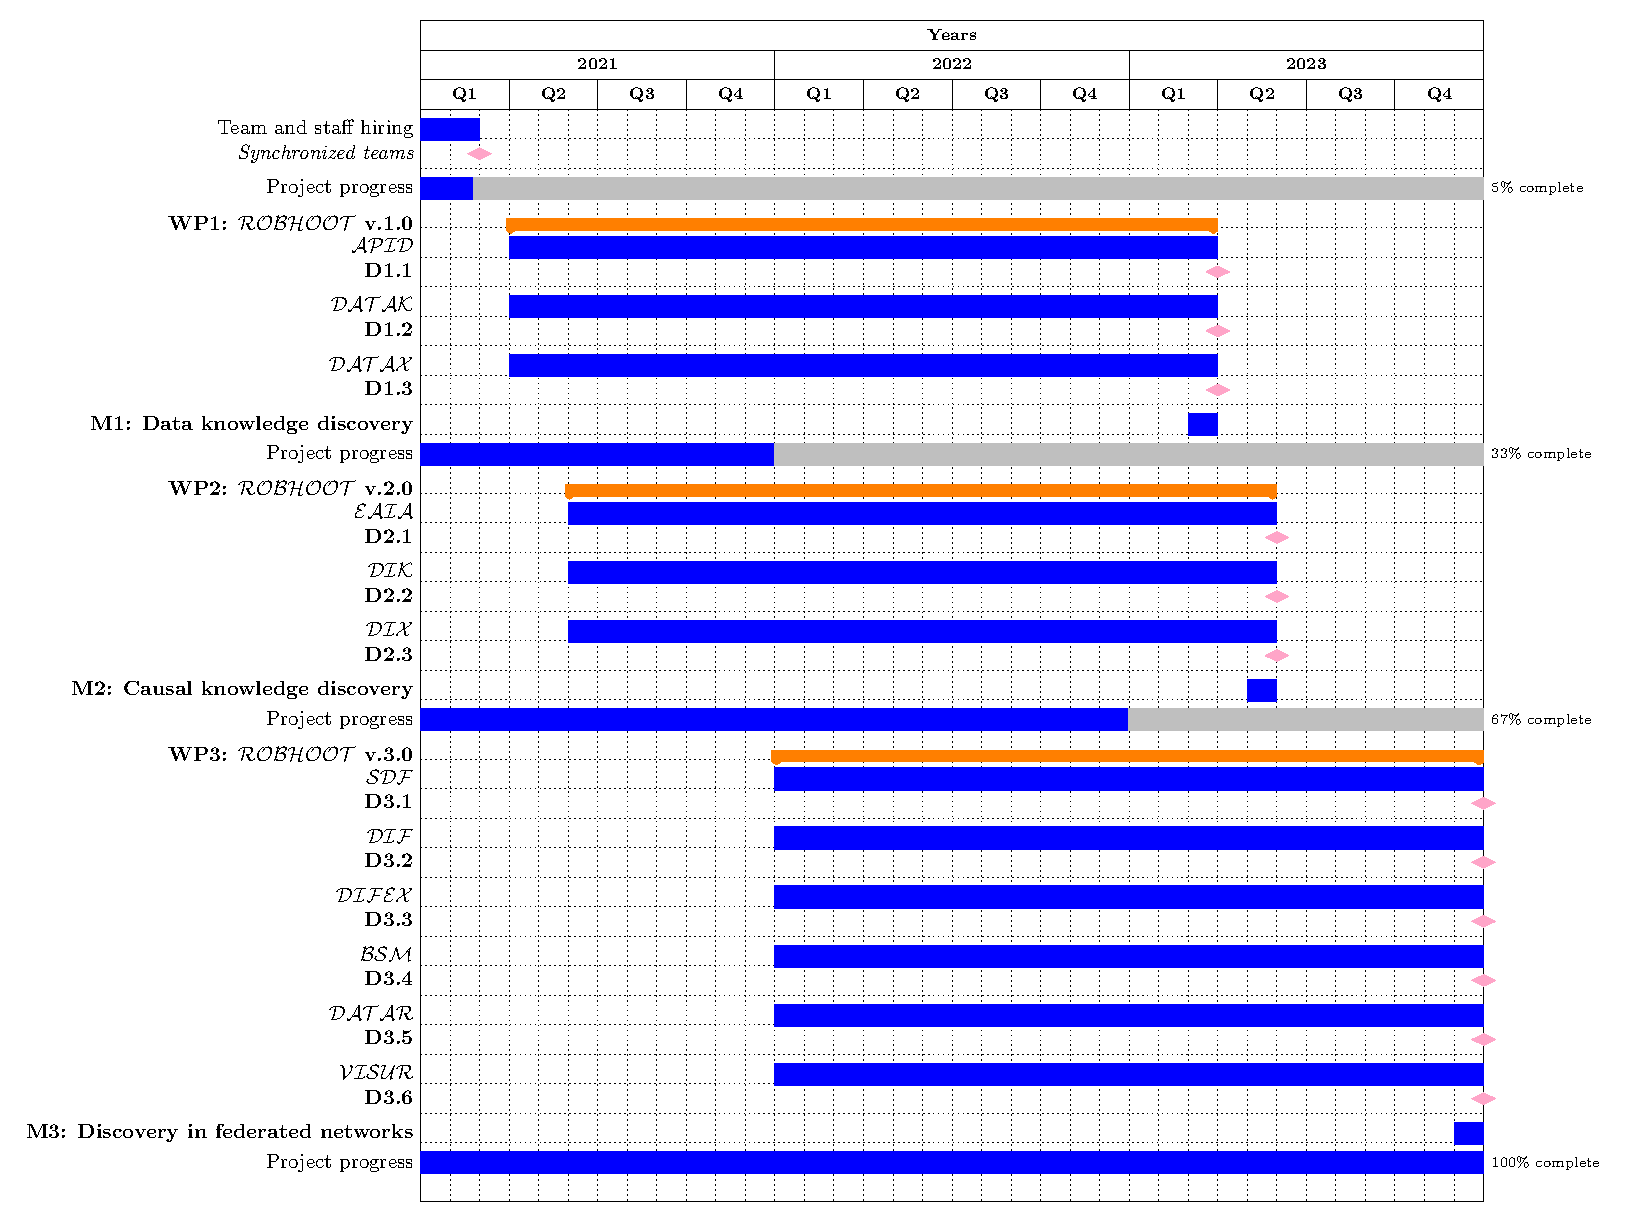
\includegraphics[width=1\textwidth]{Figures/GanttChart.pdf}
   \caption*{{\small {\bf Table 3.1a: $\mathcal{ROBHOOT}$ Gantt
         Chart}: Work package one, {\bf WP1}, introduces Milestone
       {\bf $\mathcal{ROBHOOT}$ v.1.0} and deliverables {\bf D1.1} to
       {\bf D1.3} to generate the data knowledge graph for the
       Exploration of the Seas Network (Figure 2). Work package two,
       {\bf WP2}, introduces {\bf $\mathcal{ROBHOOT}$ v.2.0} and
       deliverables {\bf D2.1} to {\bf D2.4} to fussion data and
       causal knowlede graphs into interpretable patterns, the
       discovery-knowledge graphs for the Exploration of the Seas
       Network. Work package three, {\bf WP3}, introduces {\bf
         $\mathcal{ROBHOOT}$ v.3.0} and deliverables {\bf D3.1} to
       {\bf D3.3} to discover knowledge graphs from biology-inspired
       evolving federated networks.}}
\end{figure}

  
\subsection{Research methodology and work plan , work packages,
  deliverables}

\subsubsection{{\bf WP1: $\mathcal{ROBHOOT}$ v.1.0}: \\ Data Knowledge
  Graphs}

Heterogeneous API discovery technologies to build robust and scalable
automated interpretable data-driven discovery is an existing need
\citep{Fan2012,Staar2018}. They are particularly relevant to generate
explainable (or interpretable) Artificial Intelligence technologies
for global emergency or sustainability landscapes where new questions
and scenarios are constantly emerging \citep{Futia2020}. Data
heterogeneity, however, comprises a series of privacy requirements,
formats, dimensions, biases and spatiotemporal resolution
\citep{Openstreetmap,Bluecloud,HOT,Elixir}. Fortunately, standard
protocols to automate API access, semantic knowledge extraction, and
ETFs algorithms are rapidly advancing
\citep{Fan2012,APISGURU,OpenKnowledgeFoundation}. On the other side,
new algorithms with different types of semantic technologies are
rapidly emerging in the context of building data knowledge graphs from
multiple datasets \citep{KGcovid19}. Yet, technologies focusing on
(novel) evolutionary semantic algorithms to build data knowledge
graphs from many heterogeneous API and data-sources that can be
rapidly integrated into interpretable technologies are not currently
in place \citep{Futia2020}. $\mathcal{ROBHOOT}$ v.1.0 explores
science-enabled technologies around heterogeneous API data-discovery
along three main deliverables (Table 3.1a-b, {\bf D.1.1} to {\bf
  D.1.3} and Figure 3). $\mathcal{ROBHOOT}$ v.1.0 generates a data
knowledge graph from heterogeneous data-sources for the exploration of
the Seas network, a database initially containing 9 million entries,
1612 species, around 20 countries and 11 sampling methods (Figure 2).
      
 %Word package description
\begin{table}[h!]
\begin{center}
  \begin{tabular}{|m{3cm} || m{12cm} || m{1cm}|}
    \hline\hline\hline
    \rowcolor{lightpink!30}
    {\bf Work package} & & {\bf Lead Beneficiary} \\
    \hline
    \rowcolor{piggypink!20}
    {\bf Title} & {\bf $\mathcal{ROBHOOT}$ v.1.0} &  \\
    \hline
    \rowcolor{piggypink!20}
    {\bf Participants} & {\bf Fortuna, Egu\'iluz, Choirat} & \\
    \hline
    \rowcolor{piggypink!20}
    {\bf Person Month per participant} & & \\
    \hline
    \rowcolor{piggypink!20}
    {\bf Start month} & {\bf 3} & \\
    \hline
    \rowcolor{piggypink!20}
    {\bf End month} & {\bf 27} & \\
    \hline
    \rowcolor{piggypink!20}
    {\bf Objectives} & Data Knowledge Graph & \\
    \hline
    \rowcolor{piggypink!20}
    {\bf Description} & Extraction diverse data-sources to infer data knowledge graphs & \\
    \hline
    \rowcolor{piggypink!20}
    {\bf Deliverables} & {\bf D1.1 ($\mathcal{APID}$}): Heterogeneous API and data discovery
                         {\bf D1.2 ($\mathcal{DATAK}$}): Heterogeneous data knowledge graph
                         {\bf D.1.3 ($\mathcal{DATAX}$}): Data knowledge graph for the exploration of the Seas network & \\
    \hline\hline\hline
    \rowcolor{piggypink!20}
    {\bf Title} & {\bf $\mathcal{ROBHOOT}$ v.2.0} &  \\
    \hline
    \rowcolor{piggypink!20}
    {\bf Participants} & {\bf Baity, Guimer\`a, Meli\'an, Vicente} & \\
    \hline
    \rowcolor{piggypink!20}
    {\bf Person Month per participant} & & \\
    \hline
    \rowcolor{piggypink!20}
    {\bf Start month} & {\bf 5} & \\
    \hline
    \rowcolor{piggypink!20}
    {\bf End month} & {\bf 29} & \\
    \hline
    \rowcolor{piggypink!20}
    {\bf Objectives} & Causal Knowledge Graph & \\
    \hline
    \rowcolor{piggypink!20}
    {\bf Description} & Interpretable knowledge extraction from data knowledge graphs & \\
    \hline
    \rowcolor{piggypink!20}
    {\bf Deliverables} & {\bf D2.1 ($\mathcal{EAIA}$}): Automated biology-inspired AI algorithms        
                         {\bf D2.2 ($\mathcal{DIK}$}): Discovery evolutionary biology-inspired knowledge graphs
                         {\bf D2.3 ($\mathcal{BSM}$}): Bayesian causal-knowledge graphs                
                         {\bf D2.4 ($\mathcal{DIX}$}): Discovery knowledge graphs for the exploration of the Seas network  & \\
    \hline \hline\hline
    \rowcolor{piggypink!20}
    {\bf Title} & {\bf $\mathcal{ROBHOOT}$ v.3.0} &  \\
    \hline
    \rowcolor{piggypink!20}
    {\bf Participants} & {\bf von Waldow, Maass} & \\
    \hline
    \rowcolor{piggypink!20}
    {\bf Person Month per participant} & & \\
    \hline
    \rowcolor{piggypink!20}
    {\bf Start month} & {\bf 18} & \\
    \hline
    \rowcolor{piggypink!20}
    {\bf End month} & {\bf 42} & \\
    \hline
    \rowcolor{piggypink!20}
    {\bf Objectives} & Biology-inspired Evolving Federated Network & \\
    \hline
    \rowcolor{piggypink!20}
    {\bf Description} & Automated discovery knowledge graphs in federated networks & \\
    \hline
    \rowcolor{piggypink!20}
    {\bf Deliverables} & {\bf D3.1 ($\mathcal{SDF}$}): Sharing discovery knowledge graphs in federated networks
                         {\bf D3.2 ($\mathcal{DIF}$}): Discovery in biology-inspired federated networks 
                         {\bf D2.3 ($\mathcal{DIFX}$}): Discovery in biology-inspired exploration of the Seas federated networks  & \\
    \hline\hline\hline
  \end{tabular}
\end{center}
\caption*{{{\bf Table 3.1b Work package description}: Work package,
    Title, Participants, Person Months per participant, Start and End
    month, Objectives, Description and deliverables of each Work
    Package.}}
\end{table}


\subsubsection{{\bf WP2: $\mathcal{ROBHOOT}$ v.2.0}: \\
  Causal Knowledge Graphs}

AI is rapidly advancing in automated discovery (i.e., AutoML
\citep{Real2020}) and becoming a more explainable or interpretable
technology making more transparent the processes underlying the
discovery \citep{Gil2019,Futia2020}. While automated and explainable
discovery methods are rapidly advancing \citep{Guimera2020, ++ refs},
evolutionary biology-inspired methods to infer mechanistic
understanding of complex problems are not currently in place
(ref). Evolutionary biology-inspired techniques offer ruled-based
evolution of heterogeneous agents forming network of interactions to
disentangling complex sustainability problems (Figure 2). Evolutionary
dynamics explores open-ended language of models with varying
biologically relevant functions like code insertions, deletions,
inversions and other molecular and genotype-phenotype processes to
search for biologically inspired solutions in multidimensional systems
to decipher complex empirical patterns.

In this regard, causal knowledge graphs connect automated and
explainable AI throughout prediction and knowledge power (Figure
2). Automated and interpretable data inference still present many
challenges in the context of multidimensional landscapes
\citep{OHare2015,Cranmer2019}. This is particularly relevant in Earth
and Ecosystem science and Biodiversity and Sustainability science
\citep{Reichstein}, where merging automation to interpretable data
might increase human ability to make stronger inferences about future
sustainability challenges and solutions. $\mathcal{ROBHOOT}$ v.2.0}
explores science-enabled technologies around multidimensional
landscapes developing open-ended automated modeling, evolutionary
biology-inspired solutions, AI methods and Bayesian space models along
four main deliverables (Table 3.1a-c, {\bf D.2.1} to {\bf D.2.4} and
Figure 3). In order to make inference from complex data more robust we
contrast predictions from Evolutionary biology-inspired algorithms in
the framework of automated Bayesian machines to explore open-ended
language of models ensuring the search, the evaluation of models,
trading-off complexity, fitting to the data and quantify resource
usage \citep{Guimera2020,Steinruecken}. $\mathcal{ROBHOOT}$ v.2.0
deploys milestone Evolutionary automation (Figure 3.1c) for the
discovery knowledge graph for the exploration of the Seas (Figure 2)
containing 9 million entries, 1612 species, X countries and Y sampling
methods.

   \vspace{-0.15 in}
   \begin{figure}[h!]
     \centering
     \hspace{-0.5 in}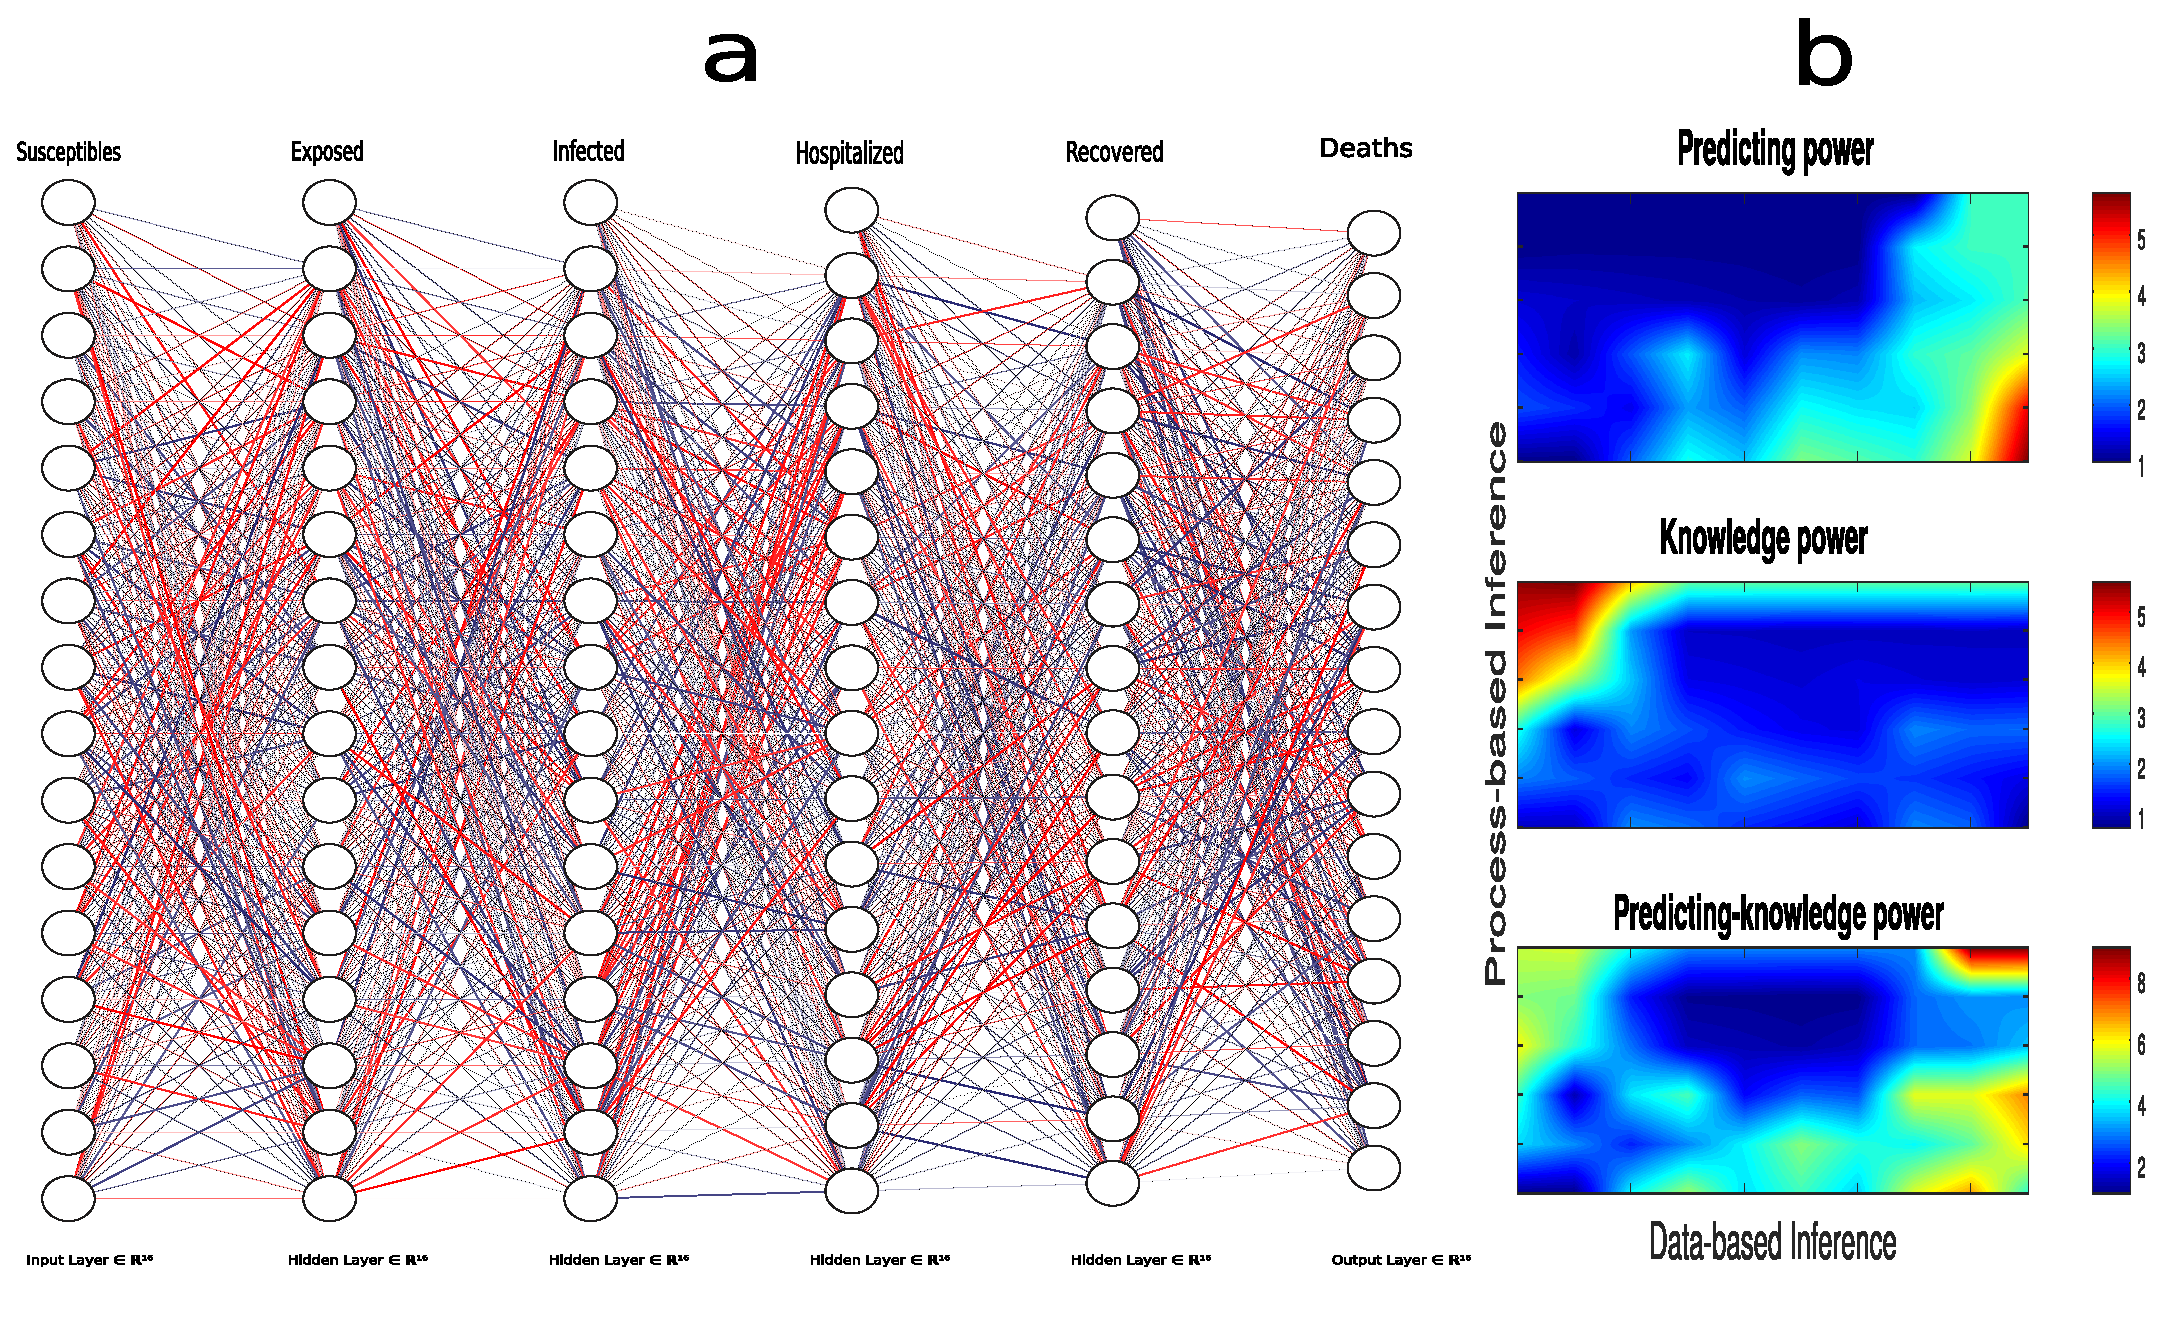
\includegraphics[width=18cm,height=16cm]{Figures/Figure3integrated.pdf}
     \caption*{\small {\bf Figure 2: Causal Knowledge Graphs}.  {\bf
         Top}) The Irish Ground Fish Survey (IE-IGFS, Orange) and the
       Spanish Survey on the Porcupine Bank (SP-PORC, Blue) were part
       of the 2018 International Bottom Trawl Survey, coordinated by
       the International Council for the Exploration of the Sea
       \citep{ices}. Ireland and Spain use different Gears: The GOV
       gear has a larger vertical opening (Ireland, 3-4 m) respect to
       the Baka used on the Porcupine Bank (Spain, 2-3 m). This makes
       catchability different for different fish species, such as
       megrim ($Lepidorhombus$ $whiffiagonis$, {\bf Center left}) and
       haddock ($Melanogrammus$ $aeglefinus$, {\bf Center right}), in
       which both countries have very different commercial
       interests. Haddock is a species of the cod family, highly
       prized in northern Europe, while megrim is a species of
       flatfish, consumed largely in Spain and France. Spain catches
       megrim better than haddock and viceversa for Ireland. This
       generates a strong bias in the distribution maps (compare
       Megrim vs. Haddock map, Center). {\bf Bottom left}
       Causal-Knowledge Graph representing the 2-countries, 2-species
       and 2 gears example. The whole data set for 2018 contains 11
       countries, 461 fish especies (approx. 200k individuals
       sampled), and 5 gears. {\bf Bottom right} Predictive-knowledge
       power map. x-axis represents ``Data-based inference'' (i.e.,
       gradient of non-interpretable ML methods from left (low) to
       right (high) predicting power). y-axis represents
       ``Process-based inference'' (i.e., gradient of process-based
       methods from bottom (low) to top (high) knowledge power). The
       gradient of predicting power map (top) shows a hot spot red
       area in the bottom right highlighting the region where AI best
       predict the empirical data. The gradient of knowledge power map
       (middle) shows a red hot spot in the top left highlighting the
       region where the best mechanistic understanding occur. The
       predicting-knowledge power map (bottom) shows the sum of the
       two previous maps highlighting a red hot spot where predicting
       and knowledge power occur.}}
\end{figure}


%Deliverable table  
\begin{table}[h!]
\begin{center}
  \begin{tabular}{|m{2cm} || m{1.25cm} || m{1.75cm} || m{1.55cm} || m{2.4cm} || m{1.7cm} || m{1.15cm} || m{1.7cm}|}
  \hline\hline
  \rowcolor{lightpink!30}
  {\bf $\mathcal{ROBHOOT}$ v.X.X} & {\bf Deliver. number} & {\bf Deliver. name} & {\bf WP} & {\bf Name Lead} & {\bf Type} & {\bf Disem.} & {\bf Delivery date} \\
  \hline\hline
  \rowcolor{piggypink!20}
  {\bf v.1.0} & {\bf D1.1} & $\mathcal{APID}$ & WP1 & {\bf Fortuna} & OT & PU & 27 \\
  \hline\hline
  \rowcolor{piggypink!20}
  {\bf v.1.0} & {\bf D1.2} & $\mathcal{DATAK}$ & WP1 & {\bf Egu\'iluz} & OT & PU  & 27 \\
  \hline\hline
  \rowcolor{piggypink!20}
  {\bf v.1.0} & {\bf D1.3} & $\mathcal{DATAX}$ & WP1 & {\bf Leads M1} & R,OT,DEC & PU  & 28 \\
    \hline\hline
 \rowcolor{piggypink!40}
  {\bf v.2.0} & {\bf D2.1} & $\mathcal{EAIA}$ & WP2 & {\bf Meli\'an} & OT & PU & 29 \\
  \hline\hline
  \rowcolor{piggypink!40}
  {\bf v.2.0} & {\bf D2.2} & $\mathcal{DIK}$ & WP2 & {\bf Baity/Vicente} & OT & PU  & 29 \\
  \hline\hline
   \rowcolor{piggypink!40}
  {\bf v.2.0} & {\bf D2.3} & $\mathcal{BSM}$ & WP2 & {\bf Guimer\`a} & OT & PU  & 29 \\
  \hline\hline
  \rowcolor{piggypink!40}
    {\bf v.2.0} & {\bf D2.4} & $\mathcal{DIX}$ & WP2 & {\bf Leads M2} & R,OT,DEC & PU & 30 \\
    \hline\hline
   \rowcolor{piggypink!60}
  {\bf v.3.0} & {\bf D3.1} & $\mathcal{SFN}$ & WP3 & {\bf von Waldow} & OT & PU & 42 \\
  \hline\hline
   \rowcolor{piggypink!80}
  {\bf v.3.0} & {\bf D3.2} & $\mathcal{DIF}$ & WP3 & {\bf Maass} & OT & PU & 42 \\
  \hline\hline
  \rowcolor{piggypink!80}
  {\bf v.3.0} & {\bf D3.3} & $\mathcal{DIFX}$ & WP3 & {\bf Leads M3} & R,OT,DEC & PU & 42 \\
\hline\hline
  \end{tabular}
\end{center}
\caption*{{{\bf Table 3.1c List of Deliverables}: {\bf
      $\mathcal{ROBHOOT}$} contains three main work packages: {\bf
      $\mathcal{ROBHOOT}$ v.1.0} span from Month 3 to 27. Deliverable
    {\bf D1.3 ($\mathcal{DATAX}$)} generates the data knowledge for
    the exploration of the Seas network. Milestone {\bf
      $\mathcal{ROBHOOT}$ v.2.0} span from Month 5 to 29. Deliverable
    {\bf D2.4 ($\mathcal{DIX}$)} generates the discovery knowledge
    graph for the exploration of the Seas network, and {\bf
      $\mathcal{ROBHOOT}$ v.3.0} span from Month 18 to 42, bringing
    the deliverable {\bf D3.3 (DIFX)}, discovery in biology-inspired
    exploration of the Seas network.}}
\end{table}

 
\subsubsection{{\bf WP3: $\mathcal{ROBHOOT}$ v.3.0}: \\
  Discovery Knowledge Graphs in Biology-Inspired Federated Networks}

Discovery knowledge graphs are not enough if they only represent
isolated contributions and can not ``learn to learn'' among
heterogeneous groups in a biology-inspired federated network. In this
regard, federated objects can be seen as ``neural networks''
containing many types of heterogeneous nodes with varying degrees of
heterogeneity, connectivity and firing probabilities
\citep{Maass2014,Maass2015}. Technologies in digital ecosystems around
heterogenous federated networks are scarce and mostly focus on
decentralization. Decentralization technologies are rapidly advancing
in a variety of sectors. Most progress is coming from the scalability
and security fronts
\citep{Golem2016,Dilley2016,Durov2017,Androulaki2018,OceanProtocolFoundation2018,BigchainDBGmbH2018}. In
the science ecosystem, only a few applications of open decentralized
technologies exist \citep{Gunther2018}. Yet, sharing reproducible data
and causal knowledge graphs, the discovery knowledge graphs, along
biology-inspired federated networks to facilitate forecasting when
heterogeneous groups interchange information is currently not in
place.

Our understanding of the outcomes from evolved information processing
systems formed by highly heterogeneous groups, a kind of large-scale
meta-learning in the federated setting \citep{Dilley2016}, is
currently quite limited. Therefore, new science-enabled approaches
accounting for information processing with diversification of
heterogeneous and highly dimensional systems in federated networks are
required to develop science-enabled technologies where heterogeneous
agents with different interests find (non optimal)
solutions. $\mathcal{ROBHOOT}$ v.3.0 connects discovery knowledge
graphs to biology-inspired federated netwoks to study the properties
of cooperative forecasting and strong inference in the face of global
sustainability and biodiversity challenges (Figure 2 and Table
3.1.a-c). $\mathcal{ROBHOOT}$ v.3.0} deploys sharing protocols of
discovery knowledge graphs, {\bf D3.1, $\mathcal{SFN}$}, into
biology-inspired federated networks accounting for heterogeneous
agents to infer biology-inspired solutions for the exploration of the
Seas federated network (Table 3.1a-c, {\bf D.3.1} to {\bf D.2.3}).

\begin{comment}
\begin{table*}[ht]
 %\rowcolor{pink}
\begin{tabular}{ p{3.5cm} | p{14cm}}
  \hline \hline
  \textbf{Feature} &\textbf{$\mathcal{ROBHOOT}$}\\  \hline
  Long-term vision & Global open-access to a fully reproducible knowledge-generation inspired technology \\ \hline
  Breakthrough scientific and technological target & Collapsing evidence- and research-based knowledge gaps for a sustainable knowledge-inspired society\\ \hline
  Novelty & Science-based technology emerging from targeted algorithmic discovery at the interface of multilayer networks, knowledge graphs, deep-learning, and consensus mechanisms\\ \hline
  Foundational & Neutral-knowledge inspired technology for an emerging open science of science and science-society research disciplines \\ \hline
  High-risk & Adapted to explore new terrirories into the open-science-technology-society interface ecosystem \\ \hline
  Interdisciplinarity & Hybridizing expertise from distributed computing and deep learning to multilayer networks and the ecology and evolution of natural and digital ecosystems (Table 1) \\ \hline
  \bottomrule

\end{tabular}
\caption{{\bf $\mathcal{ROBHOOT}$} features along its developmental stages.}
\end{table*}
\end{comment} 



  \begin{comment}
    %\centering
  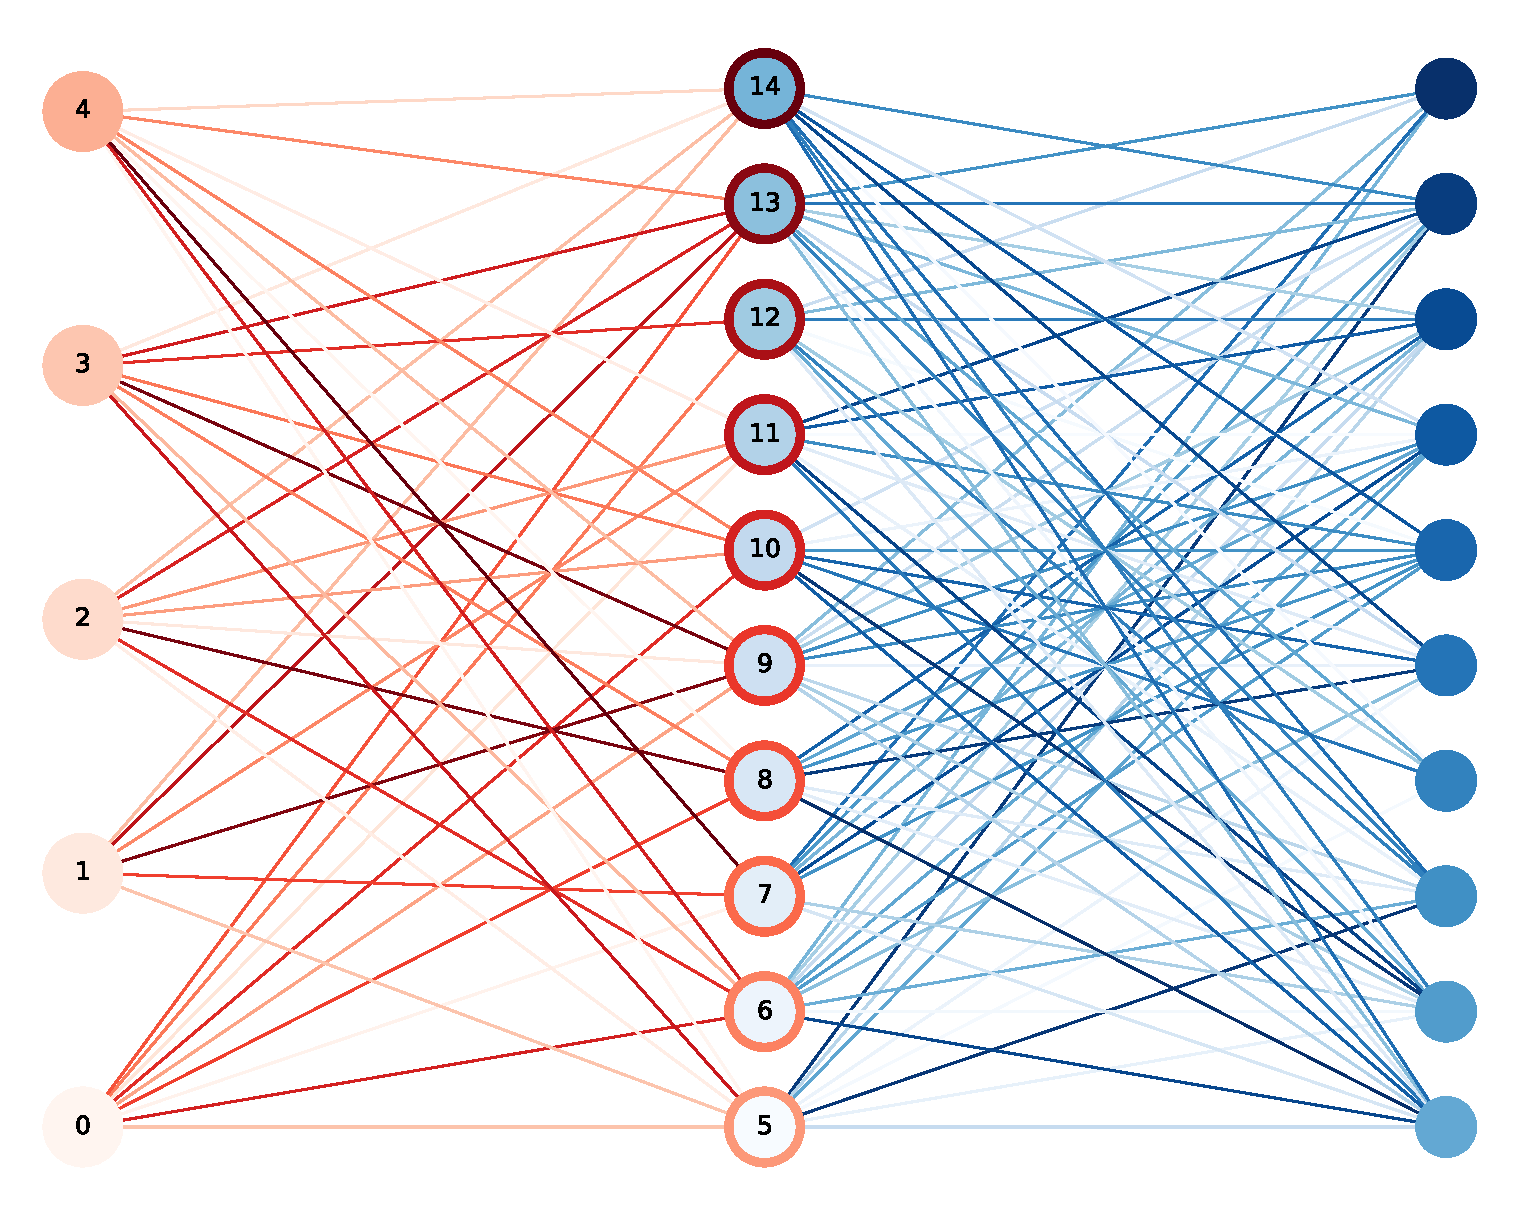
\includegraphics[width=0.45\textwidth]{Figures/FigureRobhoot.pdf}
 
  {\small {\bf Figure 3: Robhoot in Digital Ecosystems}: {\bf Left
      column}: {\bf $\mathcal{ROBHOOT}$ v.1.0} representing the
    research cycle as nodes from number 0 to 4: Data integration (0),
    Complexity Reduction (1), Inference (2), Validation (3), and
    Visualization(4)). {\bf Central column}: Nodes representing the
    research cycle in the left column are connected to open-source
    software in the digital ecosystem. Connections with node number 0
    in the left column can, for example, represent the ETLs
    open-source software interactions required to generate the {\bf
      Universal ETLs} module. The same meaning applies to the
    different nodes of the left column. {\bf Right column}: Each node
    represents a report meaning there is a reporting gradient
    generated by the connections to the open-source software from
    where each report is generated only using a subset of the research
    layers and open-source software.}
\end{comment}


\subsection{Management structure, milestones and procedures}

\begin{itemize}
  \item \textcolor{red}{Describe the organisational structure and the
      decision-making (including a list of milestones (table 3.2a))}
\item \textcolor{red}{Explain why the organisational structure and
  decision-making mechanisms are appropriate to the complexity and
  scale of the project.}
\item \textcolor{red}{Describe any critical risks, relating to project
    implementation, that the stated project's objectives may not be
    achieved. Detail any risk mitigation measures. Please provide a
    table with critical risks identified and mitigating actions (table
    3.2b) and relate these to the milestones.}
\end{itemize}

Advisory board covering the weakest parts of the proposal -- mention here



%Milestone table  
\begin{table}[h!]
\begin{center}
  \begin{tabular}{|m{1.75cm} || m{2.5cm} || m{2.5cm} || m{2.4cm} || m{6cm}|}
   \hline\hline
   \hline\hline
  \rowcolor{lightpink!30}
  {\bf Milestone number} & {\bf Milestone name} & {\bf Related work package(s)} & {\bf Due data (months)} & {\bf Verification} \\
  \hline\hline
  \rowcolor{piggypink!20}
  {\bf M1} & {\bf Discovery-Knowledge Graph}  & WP1-WP2 & 27 & OS-Software,Paper/Conf. &
  \hline\hline
  \rowcolor{piggypink!40}
  {\bf M2} & {\bf Evolutionary Automation} & WP2 & 29 & OS-Software,Paper/Conf.,demo-website &
  \hline\hline
   \rowcolor{piggypink!60}
  {\bf M3} & {\bf Cooperative Forecasting} & WP3 & 42 & OS-Software,Paper/Conf.,main-website &
  \hline\hline
  %\rowcolor{piggypink!80}
  %\bf M4} & {\bf $\mathcal{ROBHOOT}$ v.4.0} & WP4 & Months 21-42 & OS-Software,Paper/Conf.,official website &
  %\hline\hline
\hline\hline
  \end{tabular}
\end{center}
\caption*{{{\bf Table 3.2a: List of Milestones}: {\bf $\mathcal{ROBHOOT}$} contains
    three milestones: {\bf $\mathcal{ROBHOOT}$ v.1.0} span from Month
    3 to 27 to generate open-source software and research papers
    and/or conferences for the Data-Knowledge Graph. {\bf
      $\mathcal{ROBHOOT}$ v.2.0} span from Month 5 to 29 producing the
    the integration between the Data-, and the Causal-Knowledge Graph,
    the Discovery-Knowledge Graph, as a open-source software and
    research papers and/or conferences and public demo-website. {\bf
      $\mathcal{ROBHOOT}$ v.3.0} span from Month 18 to 42 to build a
    prototype of Discovery-Knowledge Graphs in Federated Cooperative
    Networks as an official {\bf $\mathcal{ROBHOOT}$} website.}}
\end{table}

  \subsection{Consortium as a whole}

  {\bf $\mathcal{ROBHOOT}$} is a science-enabled multi-feature
  technology. $\mathcal{ROBHOOT}$'s consortium is designed with a
  highly modular structure to gain milestone's functionality (Figure
  3, milestones from 1 to 3, blue, red, and pink,
  respectively). Connections among the modules reflect the emergence
  of interdisciplinarity technologies, the ``Discovery Knowledge
  Graph'', the ``Evolutionary AI Automation'' and the ``Cooperative
  Forecasting'' (Figure 3, green) \textcolor{red}{Is the
    interdisciplinarity in the breakthrough idea reflected in the
    expertise of the consortium? How do the members complement one
    another?}. {\bf $\mathcal{ROBHOOT}$ v.1.0}'s team is composed by
  Fortuna, Egu\'iluz and Choirat to bring data discovery process, to
  fully reproducible and heterogeneous knowledge graphs (section 3.1
  and Figure 3). Milestone one requires a mixture of researchers:
  computer-, data-scientists and developers and researchers working in
  complex networks from the quantitative and epistemological
  angles. Fortuna's, Egu\'iluz and Choirat's expertise complement each
  other's roles: Fortuna's team takes care of data knowledge graphs
  following evolutionary semantic algorithms for novel
  data-interactions and API discovery (i.e., {\bf $\mathcal{APID}$}
  and {\bf $\mathcal{DATAK}$, $\mathcal{DATAX}$}). Egu\'iluz's team
  focuses on network modularity, community detection and
  decentralization metrics for pattern detection in data knowledge
  graphs (i.e., {\bf $\mathcal{DATAK}$} and {\bf $\mathcal{DATAX}$},
  and Choirat's team encodes all the algorithms and procedures from
  Fortuna's and Egu\'iluz's teams into reproducible knowledge
  graphs. Milestone {\bf $\mathcal{ROBHOOT}$ v.1.0} generates a data
  knowledge graph for the exploration of the Seas (Figure 3, blue).

  {\bf $\mathcal{ROBHOOT}$ v.2.0}'s team composed by Guimer\`a, Baity,
  Vicente, and Meli\'an fussion Bayesian Machine Scientist to
  Evolutionary and AI Algorithms, forming the ``Evolutionary
  Automation'' approach (Figure 3, green). The ``Evolutionary
  Automation'' fussion data to causal knowledge graphs to make
  patterns interpretable (Figure 2). The team for this milestone add
  complementarity expertise to {\bf $\mathcal{ROBHOOT}$ v.1.0}'s team:
  Now the skills focus on data-scientists trained in deep learning
  networks and automation algorithms, theoreticians with expertise in
  Bayesian inference, and evolutionary biologists with expertise in
  evolutionary ecology theory and evolutionary-inspired networks
  (section 3.2 and Figure 3, red). Despite modules {\bf
    $\mathcal{ROBHOOT}$ v.1.0} and {\bf $\mathcal{ROBHOOT}$ v.2.0}
  focus on specific milestones and deliverables (Table 3.1a-c), they
  connect each other along data and causal knowledge graphs, the
  discovery knowledge graphs, and evolutionary automation to build a
  interdisciplinarity science-enabled technology that can be compactly
  converted into user-friendy open-software ({\bf Discovery Knowledge
    Graphs} and {\bf Evolutionary AI Automation}, green). Milestone
  {\bf $\mathcal{ROBHOOT}$ v.2.0} generates a discovery knowledge
  graph for the exploration of the Seas initially containing 9 million
  entries, 1612 species using around 11 sampling methods and more than
  15 countries (Figures 2 and 3, red). Thus, interdisciplinarity
  enters not only at the intra-module development stage, but also at
  the inter-module stage where discovery-knowledge graphs and
  evolutionary AI automation form the basis for a interdisciplinarity
  breakthrough reflected in the highly complementarity skills of the
  consortium (section 4.1). The first two modules in {\bf
    $\mathcal{ROBHOOT}$} contain researchers from Estonia, Spain,
  Switzerland and Sweden.
  
  The {\bf $\mathcal{ROBHOOT}$} consortium wants to advance the
  rapidly evolving digital ecosystem by making cooperative discovery a
  fundamental feature of it. For this purpose, a science-based
  automated and interpretable technology is not enough if each
  discovery knowledge graph stays isolated from one another. To
  contrast robustly interpretable scenarios in the face of global
  sustainability challenges, discovery knowledge graphs should learn
  to learn from heterogeneous data-sources in the contexxt of
  evolutionary biology-inspired federated networks. To achieve
  scalability for the discovery knowledge graphs, neural-inspired
  protocols in federated networks is the excellency feature of {\bf
    $\mathcal{ROBHOOT}$ v.3.0} (section 3.3). {\bf $\mathcal{ROBHOOT}$
    v.3.0}'s team composed by von Waldow and Maass, develops protocols
  for sharing discovery knowledge graphs along biology-inspired
  federated networks. The team forming {\bf $\mathcal{ROBHOOT}$ v.3.0}
  therefore requires quite a lot of contrasting skills. First,
  developers working in P2P and security protocols. Second, social
  scientists, computer scientists, and neurobiologists in
  collaboration to developers aiming to explore the role of
  heterogeneous groups of biology-inspired neurons accounting for
  heterogeneous data-sources in federated networks. Milestone {\bf
    $\mathcal{ROBHOOT}$ v.3.0} is a fundamental stepping-stone for
  developing ``Cooperative Forecasting'': it first guarantees
  discovery knowledge graphs are reproducible shareable objects. Yet,
  in the same way than evolutionary algorithms and the Bayesian
  machine scientist search automatically for open-ended space models
  to generate the plausible causal knowledge graphs, the discovery
  knowledge graphs produced in different nodes of a network need to
  automatically interact and learn from each other to find better
  forecasting scenarios at a global scale. {\bf $\mathcal{ROBHOOT}$
    v.3.0}'s implements heterogeneous groups of (cooperating and
  competing) neurons in federated networks for making cooperative
  forecasting a standard global property. Milestone {\bf
    $\mathcal{ROBHOOT}$ v.3.0} generates a discovery federated network
  for the exploration of the Seas to provide populations of scenarios
  satisfying biodiversity maintenance while guaranteeing commercial
  interest (Figure 3, pink). $\mathcal{ROBHOOT}$ v.3.0} contain
researchers from Switzerland and Austria.

\begin{figure}[h!]
  \floatbox[{\capbeside\thisfloatsetup{capbesideposition={right,top},capbesidewidth=4cm}}]{figure}[\FBwidth]
  {\caption*{Figure 3: $\mathcal{ROBHOOT}$ Consortium: {\bf
        $\mathcal{ROBHOOT}$ v.1.0} (blue) to {\bf $\mathcal{ROBHOOT}$
        v.3.0} (pink) with acronyms of each deliverable (Left column),
      tasks (Center), lead and partner names (Right columns). Links
      connect deliverables to tasks and leading/partners
      groups. $\mathcal{ROBHOOT}$ delivers three
      interdisciplinarity-driven science-enabled technologies: {\bf
        Discovery-Knowledge Graph} connecting {\bf $\mathcal{ROBHOOT}$
        v.1.0} and {\bf $\mathcal{ROBHOOT}$ v.2.0}. {\bf Evolutionary
        AI Automation} in {\bf $\mathcal{ROBHOOT}$ v.2.0}, and {\bf
        Cooperative Forecasting} connecting {\bf $\mathcal{ROBHOOT}$
        v.2.0} to {\bf v.3.0}}}
    %\label{fig:test}
  {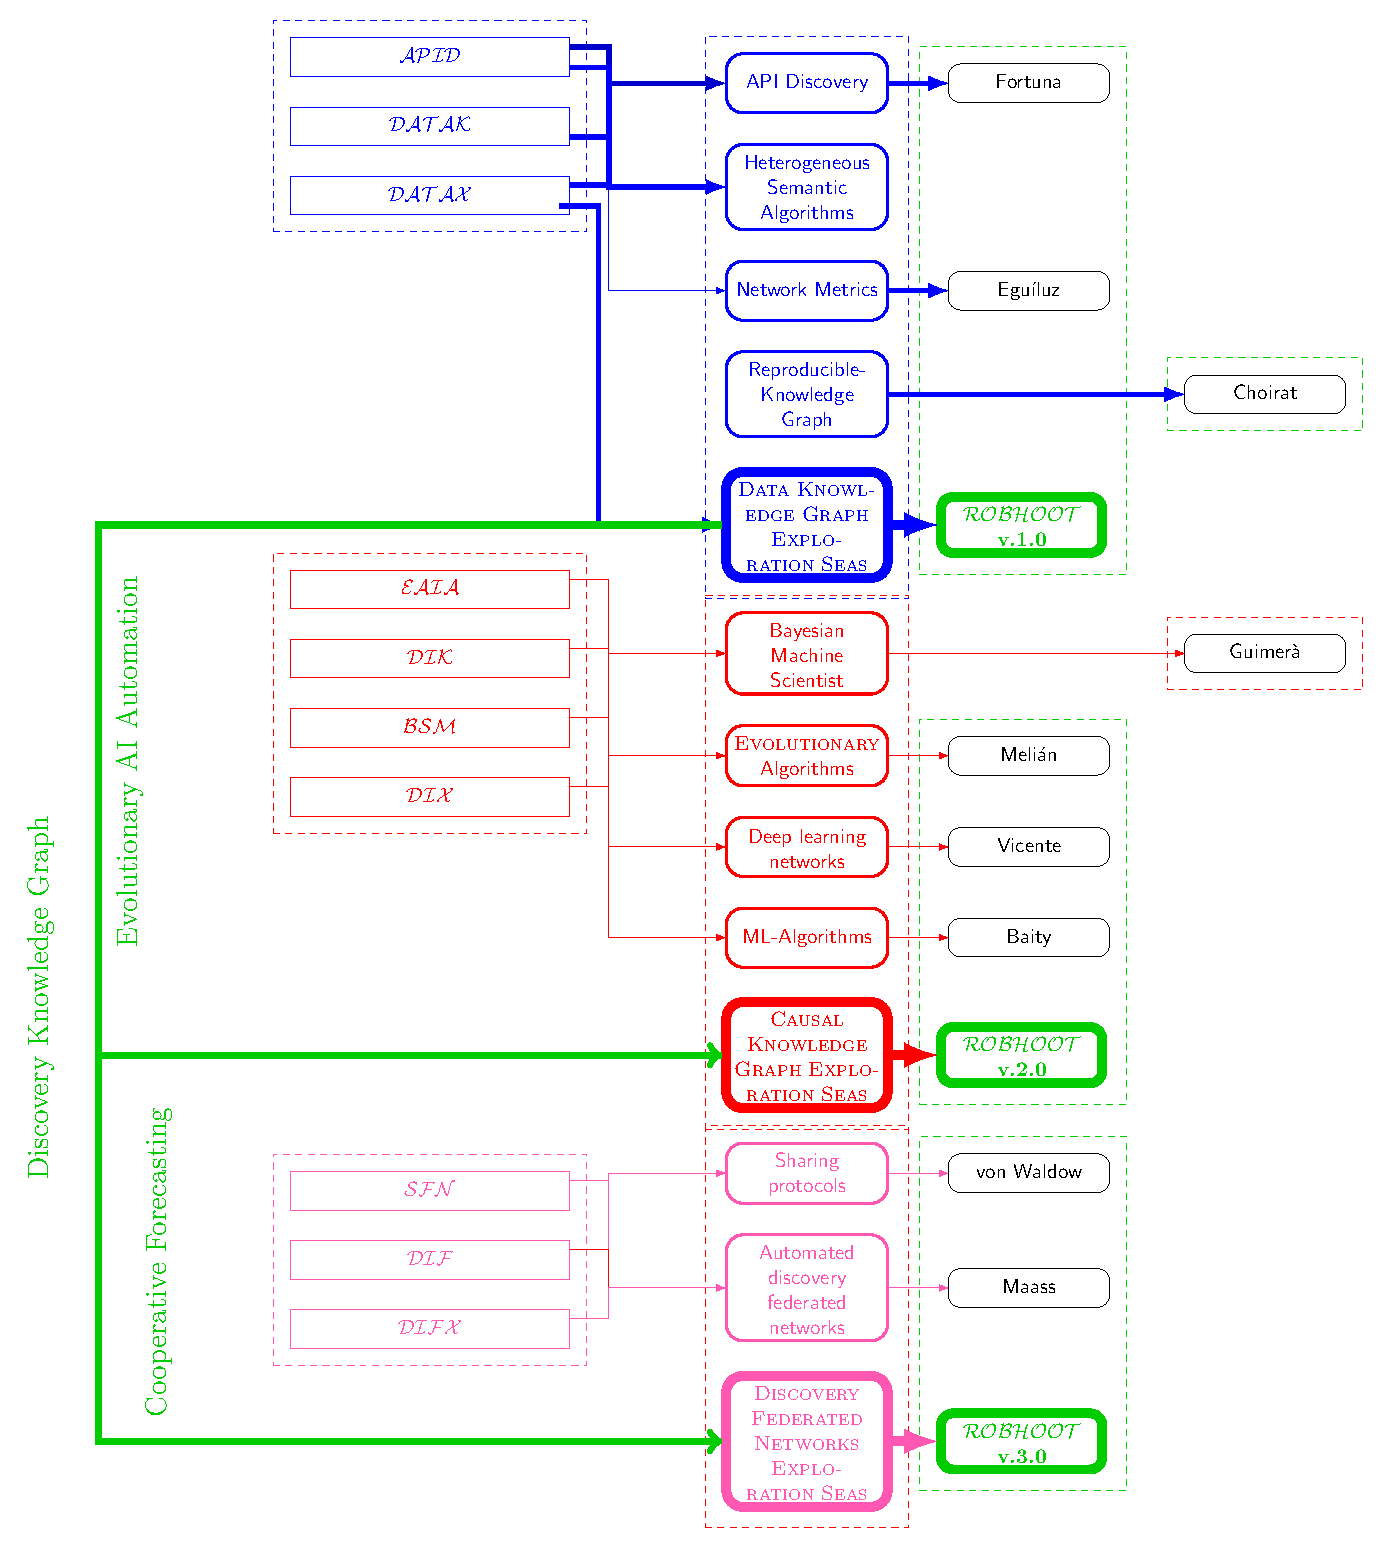
\includegraphics[width=9.75cm,height=22cm]{Figures/Consortium.pdf}}
\end{figure}
  
  
  \subsection{Resources to be committed}
 
  \begin{itemize}
  \item \textcolor{red}{Please make sure the information in this
      section matches the costs as stated in the budget table in
      section 3 of the administrative proposal forms, and the number
      of person months, shown in the detailed work package
      descriptions.  Please provide the following:}
 \item \textcolor{red}{a table showing number of person months required
    (table 3.4a)}
  \item \textcolor{red}{a table showing ‘other direct costs’ (table
      3.4b) for participants where those costs exceed 15\% of the
      personnel costs (according to the budget table in section 3 of
      the administrative proposal forms)}
\end{itemize}

  

\newpage

\section{Members of the consortium}

\begin{comment}
 This section is not covered by the page limit.

 The information provided here will be used to judge the operational
 capacity. Please make sure that you do not include information here
 that relates to the headings under sections 1 to 3. Experts will be
 instructed to ignore any information here which appears to have been
 included to circumvent page limits applying to those sections.
 \end{comment}

 \subsection{Participants (applicants)}

 \begin{itemize}
 \item \textcolor{red}{For each participant, provide the following: a
     description of the legal entity and its main tasks, with an
     explanation of how its profile matches the tasks in the proposal}
 \item \textcolor{red}{a curriculum vitae or description of the
     profile of the persons, including their gender, who will be
     primarily responsible for carrying out the proposed research
     and/or innovation activities. Indicate each person who would be a
     first-time participant to FET under Horizon 2020}
\item \textcolor{red}{a list of up to 5 relevant publications, and/or
    products, services (including widely-used datasets or software),
    or other achievements relevant to the call content}
\item \textcolor{red}{List of up to 5 relevant previous projects or
    activities, connected to the subject of this proposal}
 \item \textcolor{red}{a description of any significant infrastructure
     and/or any major items of technical equipment, relevant to the
     proposed work}
 \item \textcolor{red}{if operational capacity cannot be demonstrated
     at the time of submitting the proposal, describe the concrete
     measures that will be taken to obtain it by the time of the
     implementation of the task}
 \end{itemize}


 \begin{itemize}
 \item (description legal identity) Dr. Carlos Meli\'an is a tenured
   researcher in Theoretical Evolutionary Ecology at EAWAG, ETH-Domain
   in Switzerland, and associate professor at the University of Bern.
       (CV, gender, responsible research proposed, first time participant FET)

       He is the principal coordinator of the proposal.  Dr. Meli\'an
       has broad expertise in evolutionary algorithms and
       eco-evolutionary dynamics in ecological communities and
       biodiversity.
  
       (5 pubs)
       • Melián C, et al. 2018. Deciphering the interdependence
       between ecological and evolutionary networks. Trends in ecology
       & evolution 33,7: 504-512.  • Andreazzi C, Guimaraes P, Melián
       C. 2018. Eco-evolutionary feedbacks promote fluctuating
       selection and long-term stability of antagonistic
       networks. Proc. R. Soc. B 285: 20172596.  • Melián C, Seehausen
       O, Eguiluz V, Fortuna M, Deiner K. 2015. Diversification and
       Biodiversity Dynamics of Hot and Cold Spots. Ecography 38,
       393-401.  • Melián C, et al. 2015. Dispersal dynamics in food
       webs. American Naturalist 185, 2: 157-168.  • Melián C., et
       al. 2014. Individual trait variation and diversity in food
       webs. Advances in Ecological Research. Vol. 50. Academic Press,
       207-241.



 \item {\bf Victor M. Egu\'iluz (IFISC, CSIC, Spain)}: IFISC is an
   Maria de Maetzu Excellent center at the UIB, Balearic
   Islands. Dr. Egu\'iluz has expertise in health-related topics, in
   particular he has developed collaborations with Harvard medical
   school and many biodiversity and sustainability research
   institutions. The group of the PL has worked in the development of
   data-driven agent-based networks in social, biological and
   environmental problems with particular relevance in epidemiological
   networks.
\item
\item
   \end{itemize}

 
 \subsection{Third parties involved in the project (including use of third party resources)}


\begin{itemize}
\item \textcolor{red}{For each participant, does the participant plan
    to subcontract certain tasks (please note that core tasks of the
    project should not be sub-contracted) Y/N If yes, please describe
    and justify the tasks to be subcontracted}
\item \textcolor{red}{Does the participant envisage that part of its
    work is performed by linked third parties2 Y/N If yes, please
    describe the third party, the link of the participant to the third
    party, and describe and justify the foreseen tasks to be performed
    by the third party}
\item \textcolor{red}{Does the participant envisage the use of
    contributions in kind provided by third parties (Articles 11 and
    12 of the General Model Grant Agreement) Y/N If yes, please
    describe the third party and their contributions}
\item \textcolor{red}{Does the participant envisage that part of the
    work is performed by International Partners3 (Article 14a of the
    General Model Grant Agreement)?  Y/N If yes, please describe the
    International Partner(s) and their contributions.}
\end{itemize}


\section{Ethics and Security}

 This section is not covered by the page limit.

\subsection{Ethics}


\textcolor{red}{ For more guidance, see the document "How to complete
  your ethics self-assessment".  If you have entered any ethics issues
  in the ethical issue table in the administrative proposal forms, you
  must:}

\begin{itemize}
\item \textcolor{red}{submit an ethics self-assessment, which:}
\item \textcolor{red}{describes how the proposal meets the national
    legal and ethical requirements of the country or countries where
    the tasks raising ethical issues are to be carried out;}
\item \textcolor{red}{explains in detail how you intend to address the
    issues in the ethical issues table, in particular as regards:
    research objectives (e.g. study of vulnerable populations, dual
    use, etc.)  ▪ research methodology (e.g. clinical trials,
    involvement of children and related consent procedures, protection
    of any data collected, etc.)}
\item \textcolor{red}{the potential impact of the research (e.g. dual
    use issues, environmental damage, stigmatisation of particular
    social groups, political or financial retaliation,
    benefit-sharing, misuse, etc.)}
\item \textcolor{red}{provide the documents that you need under
    national law(if you already have them), e.g.: ◦ an ethics
    committee opinion; ◦ the document notifying activities raising
    ethical issues or authorising such activities If these documents
    are not in English, you must also submit an English summary of
    them (containing, if available, the conclusions of the committee
    or authority concerned).

    \\
    If you plan to request these documents specifically for the project
  you are proposing, your request must contain an explicit reference
  to the project title.}

\subsection{Security}


\textcolor{red{Please indicate if your project will involve:}

\begin{itemize}
\item \textcolor{red}{activities or results raising security issues:
    (YES/NO)}
\item \textcolor{red}{EU-classified information as background or
    results: (YES/NO)}
\end{itemize}  



%----------------------------------------------------------------------------------------
%	BIBLIOGRAPHY
%----------------------------------------------------------------------------------------

%\printbibliography[title={Bibliography}] % Print the bibliography, section title in curly brackets

\newpage
\bibliographystyle{unsrtnat}
%\bibliographystyle{tree.bst}
\bibliography{Robhoot.bib}

%----------------------------------------------------------------------------------------

\end{document}
